\documentclass[a4paper]{report}
\usepackage[T1]{fontenc}
\usepackage[utf8]{inputenc}
\usepackage[spanish]{babel}
\usepackage{amsmath}
\usepackage{blkarray}
\selectlanguage{spanish}
\usepackage{url}
\usepackage[document]{ragged2e}
\usepackage{graphicx}
\usepackage{cite}
\usepackage{babelbib}
\usepackage{float}
\graphicspath{ {images/} }

\title{
	{\Huge Proyecto Final}\\
	{\Huge Interpretación de bioseñales para uso en aplicaciones interactivas}
	{\large Instituto Tecnológico de Buenos Aires}\\~\\
	{
\includegraphics{itba.png}}
}

\author{{Federico Tedin} \\ {Javier Fraire}}
\date{Febrero 2017}

\makeindex

\begin{document}
\maketitle

\chapter*{Resumen}
\justifying
Las bioseñales consisten en señales producidas por tejidos vivos. Algunos ejemplos de bioseñales, en seres humanos, son: EEG (Electroencefalografía) la cual consiste en la actividad bioeléctrica cerebral, EMG (Electromiografía), la cual contempla la actividad eléctrica generada por los músculos del cuerpo, y ECG (Electrocardiograma), la cual representa la actividad eléctrica del corazón.

Dichas señales, luego de ser leídas, fueron procesadas para eliminar ruido y para extraer las características de interés. Con las características extraídas se utilizaron clasificadores para determinar si el usuario realizó una determinada acción. En este caso, se utilizó para deteterminar si el usuario estaba con los ojos abiertos o cerrados, y para determinar si el usuario estaba haciendo fuerza con la mano o no.

Con la información obtenida de los clasificadores se realizaron alteraciones en universos 3D dandolé una mayor inmersión a los usuarios.


\tableofcontents

\chapter{Estado del Arte}
En este capítulo se presentará el estado del arte en lo que respecta a los distintos usos de las bioseñales. Se brindarán algunos ejemplos del uso de las bioseñales en distintos campos.

\section{\acrshort{acat}}

La computadora utilizada por Stephen Hawking es tal vez el caso más conocido de la utilización de bioseñales en Accesibilidad. Stephen Hawking cuenta con esclerosis lateral amiotrófica, por lo que se encuentra paralizado y no puede hablar. Para poder comunicarse, Intel desarrolló un sistema compuesto por una tableta y un sensor infrarojo montado sobre sus anteojos. El sensor infrarojo detecta el movimiento en su mejilla izquierda. La tableta cuenta con una plataforma de código abierto llamada \acrshort{acat}. \acrshort{acat} provee un teclado virtual en la pantalla. Utilizando el movimiento de su mejilla, Hawking, puede detener el cursor donde desea y así, escribir. Es decir, es una entrada binaria. Este también utiliza un procesador de texto con predicción de palabras que permite acelerar el proceso.  Luego, el sistema utiliza un sintetizador de voz para comunicar lo que escribió. Esta, es solo una de las aplicaciones de \acrshort{acat}. \acrshort{acat} también le permite controlar el ratón en \emph{Windows}, y así, controlar completamente la computadora para poder utilizar su correo electrónico, navegar por internet, entre otras cosas. \acrshort{acat} puede utilizar como entrada cualquier bioseñal. \cite{hawking}.

\section{Gestos Como Dispositivos de Entrada}

La \acrshort{nasa} desarrolló un sistema para controlar un avión en una simulación utilizando los movimientos musculares medidos con sensores EMG(Electromiografía). Colocaron diversos sensores sobre una manga de tela. Con ellos, adquirieron la señal y la filtraron y eliminaron el ruido. Luego extrajeron las características y reconocieron patrones en una fase de entrenamiento. Con esta información, se aplicaron patrones de reconocimiento en una simulación interactiva. Lograron controlar un avión de guerra sin utilizar una palanca de mando. Es decir, el usuario colocaba la mano como si estuviese utilizando una palanca de mando y realizaba movimientos para controlar el avión (ver figura \ref{fig:emg-flight}) \cite{emg-flight}.

\begin{figure}[H]
	\centering
    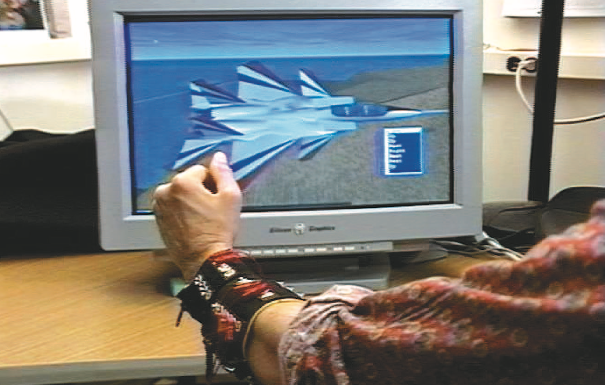
\includegraphics[width=0.8\textwidth]{emg-flight.png}
    \caption{Un usuario utilizando el dispotivo EMG para controlar un avión en una simulación  \cite{emg-flight}.}
	\label{fig:emg-flight}
\end{figure}

\section{\emph{Muscleman}}

Dos académicos de la Universidad Nacional de Seúl, utilizaron un dispositivo \acrshort{emg} y un acelerómetro para controlar un vídeojuego. Utilizando el acelerómetro, el juego era capaz de determinar si el usuario estaba dando un simple puñetazo hacia adelante, un puñetazo de abajo hacia arriba o si estaba lanzando una bola de fuego (ver figura \ref{fig:fireball}). Usando el sensor EMG, el juego medía la fuerza realizada por el usuario y la aplicaba proporcionalmente en el juego. Es decir, si el usuario realizaba poca fuerza, el ataque era débil. En cambio, si era fuerte, el ataque era fuerte. De esta forma, se utilizó como dispositivo de entrada las propias señales del cuerpo en lugar de usar un control de mando físico o el teclado \cite{emg-fireball}.

\begin{figure}[H]
    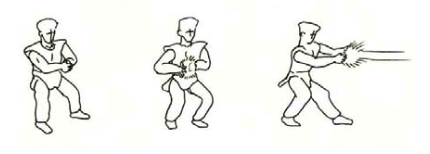
\includegraphics[width=0.8\textwidth]{emg-fireball.png}
    \caption{Movimiento que debe realiza un usuario para lanzar una bola de fuego en el videojuego \emph{Muscleman} \cite{emg-fireball}.}
	\label{fig:fireball}
\end{figure}

\section{\emph{Muse}}

La empresa \emph{Muse} desarrolló un dispositivo \acrshort{eeg} con siete electrodos. El mismo viene acompañado con una aplicación móvil que ayuda a los usuarios a meditar. Cuando el usuario tiene la mente tranquila, se escucha un clima calmo, pero cuando el usuario está alterado se escucha un clima tormentoso. Muse utiliza distintas ondas cerebrales para detectar si el usuario se encuentra relajado o no.

\section{\emph{MindFlix}}

\emph{Netflix} desarrolló \emph{MindFlix}. \emph{Mindflix} utiliza un dispositivo \acrshort{eeg} para controlar su popular servicio con la mente. Utiliza el giroscopio y el acelrómetro del dispositivo para permitirle al usuario desplazarse horizontalmente y verticalmente por la interfaz. Además, utiliza distintas ondas cerebrales para detectar cuando el usuario piensa en la palabra \emph{play}. En caso de que el usuario piense en esa palabra,  la aplicación comienza a reproducir el contenido seleccionado. Se intentó averiguar qué ondas cerebrales se utilizaban y de que forma, pero no se encontró en ningún lugar \cite{mindflix}.


\section{\emph{Neurogaming}}

\emph{Neurogaming} es la utilización de \acrshort{bci} en videojuegos para mejorar la experiencia. El concepto surgió hace algunos años pero aún no se ha explorado mucho. Existe muy pocas aplicaciones comerciales de este tipo. Un ejemplo es \emph{Throw Trucks With Your Mind} el cuál utiliza las ondas \emph{Beta} del cerebro para lanzar camiones \cite{neurogaming}.




\chapter{Marco Teórico}
Dado que este proyecto se centrará en las bioseñales, resulta fundamental explicar los conceptos necesarios para su entendimiento. Primero se hablará sobre las bioseñales. Luego se hablará sobre el procesamiento de las señales (específicamente el procesamiento de bioseñales), desde su obtención hasta la extracción de características y clasificación. Finalmente, se explicará como funcionan algunos sensores y se introducirá información teórica sobre la señal que se obtiene de los mismos.

\section{Bioseñales}\label{sec:biosignals}

Una bioseñal puede ser definida como una descripción de un fenómeno fisiológico. Como hay un gran número de mecanismos fisiológicos de interés, la cantidad de bioseñales es muy grande. Como se puede observar en la figura \ref{fig:biosignals-clasification} las bioseñales puede ser clasificadas por lo menos por tres criterios distintos \cite{biosignal-book-2}: 

\begin{itemize}
	\item \textbf{Existencia:}
		\begin{itemize}
			\item Permanentes: Existen sin necesidad de un impacto artificial, disparador o excitación externa al cuerpo y están disponibles todo el tiempo. Por ejemplo, la señal electrocardiográfica es inducida por la excitación eléctrica del corazón.
			\item Inducidas: Son disparadas artificialmente, excitadas o inducidas externamente. Su duración está ligada a la duración de la excitación. Cuando el impacto artificial termina, la bioseñal se atenúa. Por ejemplo, la pulsioximetría (SpO2) utiliza luz para detectar el oxígeno en sangre y la señal dura tanto tiempo como dicha luz se encuentre encendida.
		\end{itemize}
	\item \textbf{Dinamismo:}
		\begin{itemize}
			\item Casi estáticas:  Exhiben pocos cambios a lo largo del tiempo. Un ejemplo de esta señal es la temperatura del cuerpo.
			\item Dinámicas: Varían mucho a través del tiempo. Un ejemplo de está señal es la electrocardiografía ya que el latido del corazón cambia constantemente.
		\end{itemize}
	\item \textbf{Origen:}
		\begin{itemize}
			\item Eléctricas: Estas incluyen señales como electrocardiograma, que refleja la actividad eléctrica del corazón, electroencefalograma (EEG), que refleja la actividad eléctrica de las neuronas,  electromiografma (EMG), que refleja la actividad eléctrica de los músculos, o la respuesta galvánica de la piel (GSR), que refleja las variaciones de energía en la piel.
			\item Magnéticas: Reflejan un campo magnético inducido. Por ejemplo un magnetocardiograma utiliza los campos magnéticos emitidos por las corrientes eléctricas generadas por la excitación del corazón.
			\item Mecánicas: Incluyen deformaciones del cuerpo o vibraciones en la piel. Por ejemplo un mecanorespirograma utiliza los movimientos del abdomen para medir el ritmo cardíaco.
			\item Ópticas: Utilizan la absorción de la luz. Se utiliza una luz artificial. Un ejemplo es la pulsioxomietría (SpO2).
			\item Acústicas: Utiliza diversos sonidos del cuerpo como por ejemplo sonidos cardíacos.
			\item Químicas: Reflejan la composición química y los cambios temporales en los elementos sólidos, líquidos y gaseosos del cuerpo.
			\item Térmicas: Utilizan la absorción y pérdida de calor en el cuerpo.
			\item Otras.
	\end{itemize}
\end{itemize}

\begin{figure}[H]
	\centering
    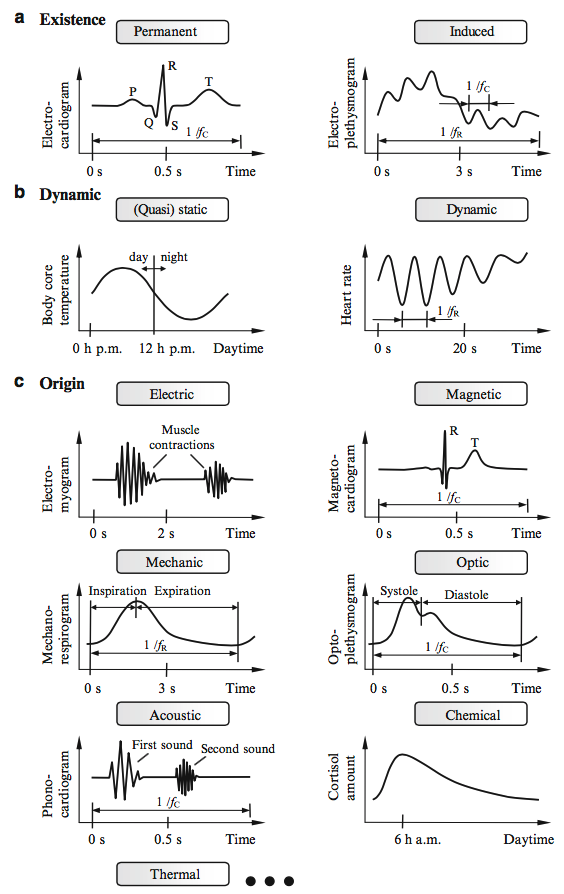
\includegraphics[width=0.8\textwidth]{biosignals-clasification.png}
    \caption{Las posibles clasificaciones de las bioseñales de acuerdo a su \textbf{(a)} existencia, \textbf{(b)} dinamismo y \textbf{(c)} origen \cite{biosignal-book-2}.}
	\label{fig:biosignals-clasification}
\end{figure}

\section{Obtención y Procesamiento de Señales}

En la figura \ref{fig:signal-pipeline} se pueden observar las distintas etapas por las que pasa una bioseñal al ser procesada: obtención de la señal fisiológica de un sensor, utilización de un transductor, procesamiento analógico, digitalización, transmisión, procesamiento de la señal digital, extracción de características y clasificación, y salida.

\begin{figure}[H]
	\centering
    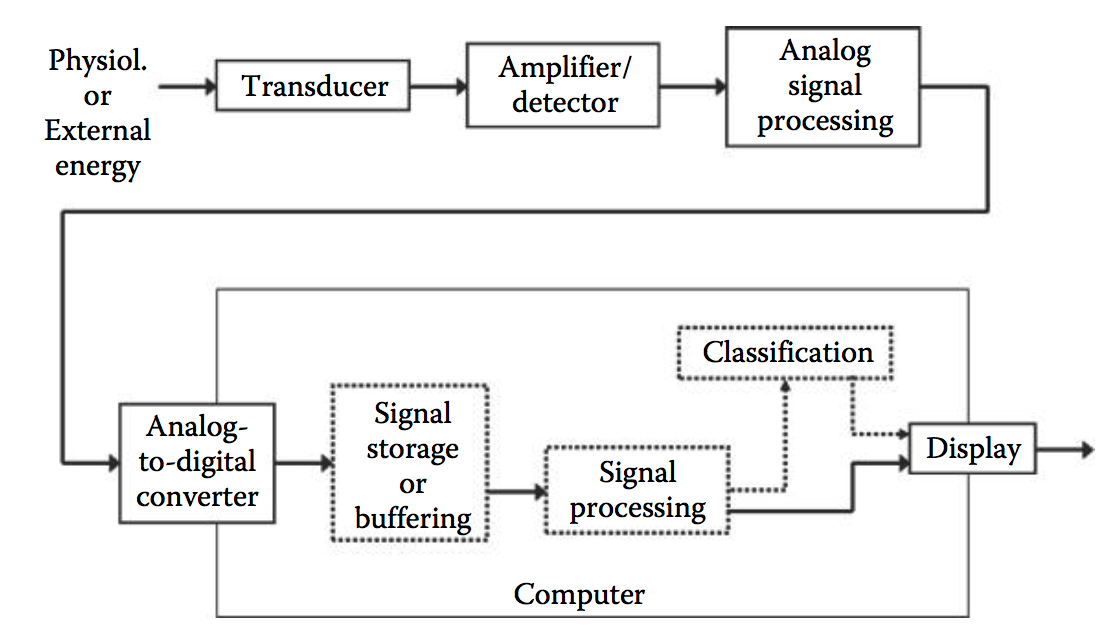
\includegraphics[width=0.8\textwidth]{signal-pipeline.png}
    \caption{Representación esquemática de las etapas del procesamiento de las bioseñales \cite{biosignal-book}.}
	\label{fig:signal-pipeline}
\end{figure}

\subsection{Obtención de la Señal Fisiológica}

Esta es la primer etapa en el procesamiento de bioseñales. Se debe obtener la señal de algún sensor. Puede ser un electrodo, un fotodetector, entre otros. La  señal viene en forma de energía. Dicha energía puede ser generada por el proceso en si (por ejemplo la actividad eléctrica producida por los músuclos), puede ser energía indirectamente relacionada al proceso o puede ser producida por una fuente externa \cite{biosignal-book}.

\subsection{Utilización de un Transductor}

Un transductor es un dispositivo que convierte energía de un tipo a otro. El propósito aquí es transferir información, no transformar energía. Se convierte la energía a energía eléctrica. Por lo general, la salida de un transductor de un biosensor es voltaje. En la figura \ref{fig:biotransducer} se puede observar una representación de un transductor. El trandsuctor es el elemento más crítico en el sistema ya que es la interfaz entre el sujeto y el resto del sistema. Este determina que tan invasivo es un dispositivo. Luego de pasar por el transductor, se utiliza un amplificador o detector \cite{biosignal-book}.

\begin{figure}[H]
	\centering
    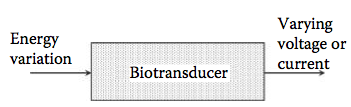
\includegraphics[width=0.8\textwidth]{biotransducer.png}
    \caption{Representación de un transductor utilizado en biosensores \cite{biosignal-book}.}
	\label{fig:biotransducer}
\end{figure}

\subsection{Procesamiento de la Señal Analógica}

La mayoría de los sensores procesan la señal analógica obtenida del transductor. El procesamiento más común es restringir el rango de frecuencias o ancho de banda utilizando filtros analógicos. Los filtros analógicos son dispositivos electrónicos que remueven un determinado rango de frecuencias. El filtrado es usualmente quien establece el ancho de banda de todo el sistema. La ganancia de un filtro es la relación entre la amplitud de la señal de salida y la amplitud de la señal de entrada define como:

$$ \textrm{Ganancia} (f) = \frac{\textrm{Valores de salida} (f)}{\textrm{Valores de entrada} (f)}  $$

Los filtros más comunes pueden observarse en al figura \ref{fig:filters} y son: 

\begin{itemize}
\item \textbf{Pasa bajos:} Atenúa las frecuencias superiores a un determinado valor. 
\item \textbf{Pasa altos:} Atenúa las frecuencias inferiores a un determinado valor. 
\item \textbf{Pasa bandas:} Atenúa las frecuencias fuera de un determinado intervalo.
\item \textbf{Supresión de bandas:} Atenúa las frecuencias dentro de un determinado intervalo \cite{biosignal-book}.

\end{itemize}

\begin{figure}[H]
	\centering
    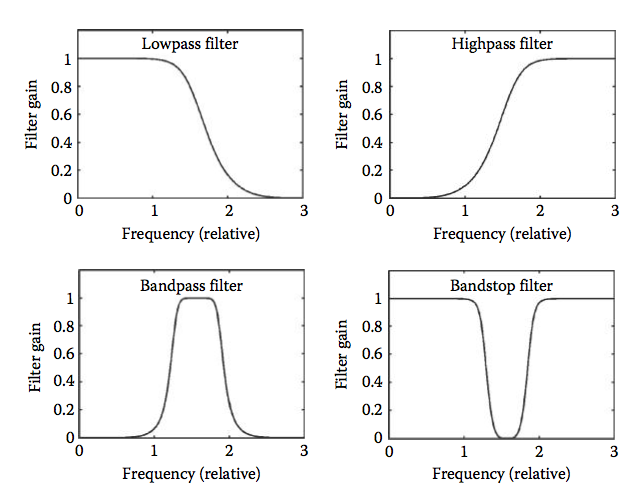
\includegraphics[width=0.8\textwidth]{filters.png}
    \caption{Influencia en la frecuencia de los filros básicos \cite{biosignal-book}.}
	\label{fig:filters}
\end{figure}

\subsection{Digitalización}

Todas las bioseñales son analógicas. Por este motivo, deben ser digitalizadas para poder ser utilizadas por una computadora. Este proceso ocurre en el dispositivo. Cuenta con un componente electrónico que convierte un voltaje analógico en número digital equivalente. Una onda continua ($ x(t) $) se convierte en una onda discreta ($x[t]$), una función de números reales que son definidos como enteros en puntos discretos en el tiempo. Estos números se conocen como muestras y los puntos discretos en el tiempo son usualmente tomados en intervalos regulares ($T$), también conocida como frecuencia de muestreo:

$$ f_{s} = \frac{1}{T_{s}}\, Hz $$

Entonces, la señal analógica es segmentada en varias partes para que pueda caber en la memoria de una computadora. Este concepto se conoce como ventana \cite{biosignal-book}. En la figura \ref{fig:digitalization} se puede observar el resultado digitalizar una señal continua.

\begin{figure}[H]
	\centering
    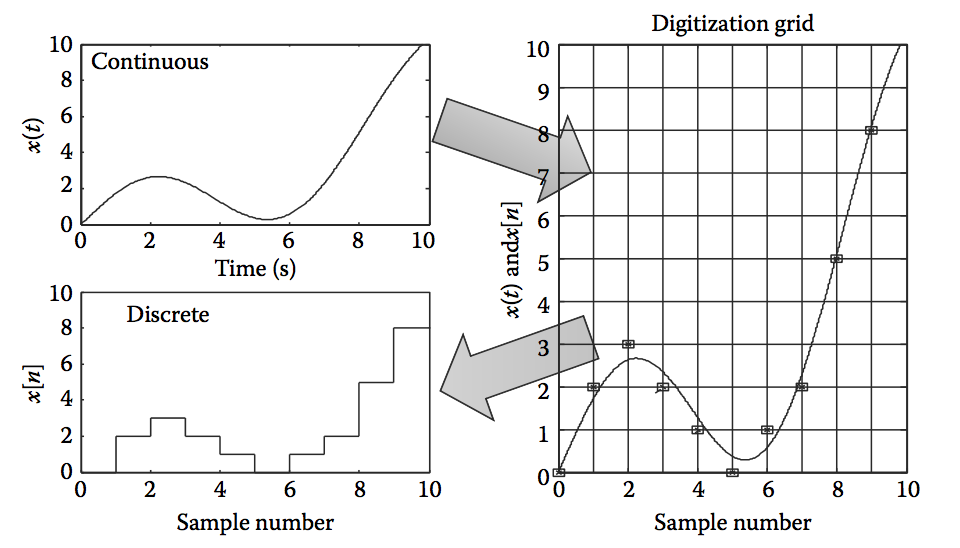
\includegraphics[width=0.8\textwidth]{digitalization.png}
    \caption{Digitalizar una señal continua, esquina superior izquierda, requiere partir la señal en tiempo y amplitud, lado derecho. El resultado es una serie de números disgretos que se aproximan a la señal, esquina inferior izquierda.  \cite{biosignal-book}.}
	\label{fig:digitalization}
\end{figure}

Digitalizar una señal implica segmentar la amplitud y el tiempo. Resulta evidente que la señal digitalizada obtenida no es igual a la analógica. El grado de aproximación de la señal digital a la analógica depende de la segmentación realizada. Como se mencionó, se segmentan las siguientes dos componentes:

\begin{itemize}
\item \textbf{Amplitud:} También se conoce como cuantificación. El grado de aproximación en este caso depende de la cantidad de valores distintos que son utilizados para representar la señal, es decir, la cantidad de bits utilizados. El nivel de cuantificación ($q$) se define como el tamaño del segmento de amplitud . El efecto de la cuantificación es la adición de ruido y este es determinado por $q$. En la figura \ref{fig:quantization} se puede observar el ruido añadido por la cuantificación. Por lo general los conversores usan $8$, $12$ y $16$ bits de salida. Pues la mayoría de las señales, no cuentan con una relación señal-ruido lo suficientemente elevada como para utilizar una resolución mayor.
\item \textbf{Tiempo:} Se refiere al muestreo. El criterio de \emph{Nyquist} establece que la frecuencia máxima (frecuencia de \emph{Nyquist}) obtenida es la mitad que la frecuencia de muestreo. El teorema de \emph{Shannon-Nyquist} establece que para poder recuperar la señal analógica a partir de la señal digital, se debe muestrear al doble que la máxima frecuencia contenida en la señal original, es decir, $ f_{s} > 2\, f_{max} $. Utilizar frecuencias de muestro más altas es innecesario e implica tener que guardar más información y tener que procesarla a una velocidad mayor .  Aún así, en la práctica es muy común que se utilicen frecuencias de muestreo de tres hasta cinco veces $f_{max}$. De esta forma se incrementa el espacio entre frecuencias y se facilita la tarea de eliminar frecuencias indeseadas \cite{biosignal-book}. Esto se debe a que se cuenta con una mayor granularidad al tratar con las frecuencias. Por ejemplo si se cuenta con una frecuencia de muestro de $128 \, Hz$, se obtienen $64$ valores al realizar la Transformada de \emph{Fourier} (en realidad son $128$ pero por simetría, solo se utiliza la mitad). Entonces, se cuenta con escalones de $2 \, Hz$, es decir, si se quiere obtener la frecuencia $ 8 Hz$, el valor en realidad representa $ 8 \, Hz - 9 \, Hz$. En cambio, si se utilizan $256 \, Hz$, el escalón es de $ 1 \, Hz$ lo que simplifica la obtención de determinadas frecuencias.
\end{itemize}

\begin{figure}[H]
	\centering
    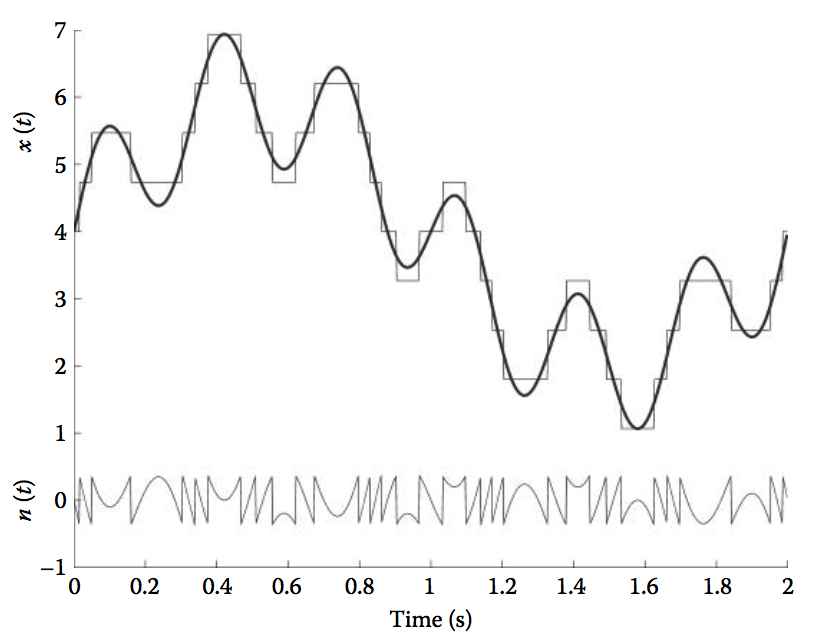
\includegraphics[width=0.8\textwidth]{quantization.png}
    \caption{El efecto de la cuantificación de la señal original puede verse como ruido añadido \cite{biosignal-book}.}
	\label{fig:quantization}
\end{figure}

\subsection{Transmisión de la Señal}\

Luego de digitalizar la señal, el dispositvo puede transmitirla hacia alguna computadora. Algunos dispositivos la utilizan directamente y no necesitan transmitirla. La transmisión puede tomar muchas formas. La señal puede ser transmitida por puerto serie, por USB, por \emph{bluetooth}, por \emph{wi-fi}, entre otros. El protocolo que se utilice para transmitir la señal depende del medio y es decisión del fabricante cuál utilizar. Por ejemplo si es un puerto serie, se transfiere bit a  bit. Luego, en la computadora debe haber un controlador que pueda recibir esta información transmitida.

\subsection{Procesamiento de la Señal Digital}

Como se mencionó anteriormente, la señal digital puede presentar ruido que se genera al digitalizarla. En algunos casos, hay que aplicar filtros para reducir el ruido. Existen diversos filtros. Uno de ellos es el filtro \emph{Gaussiano}. Dicho filtro suaviza la señal por lo que elimina los picos que se pudieran haber introducido.. Además, el filtro \emph{Gaussiano}, a diferencia de otros filtros, no elimina las altas frecuencias completamente. El filtro \emph{Gaussiano} se aplica haciendo una convolución de la señal con la siguiente función:
$$ g(x) = \frac{1}{\sqrt{2 * \pi} * \sigma } * e^{-\frac{x^{2}}{2 * \sigma^{2}}} $$

Muchas veces las señales pueden tener una cierta tendencia. Es decir, se encuentran desfasadas. Para compensar esta tendencia, se utiliza una técnica conocida como \emph{detrending}. Esta consiste en eliminar dicha tendencia.  La forma más simple de realizar \emph{detrending} es calcular la media del sensor y restarla a cada valor. Existen otros algoritmos más complejos de \emph{detrending} pero estos escapan al foco de este trabajo.

Una vez que se redujo el ruido, se pueden aplicar otros filtros o continuar. Como se mencionó anteriormente muchos sensores tienen como salida el nivel de potencial eléctrico medidas en $\mu V$ (microvoltios). Esta información sin ningún tipo de procesamiento no es útil. Dependiendo de que se quiera detectar se pueden realizar distintas operaciones. Una de ellas, es la búsqueda de picos. La primera derivada de un pico tiene un cruce descendente igual a cero en su máximo. Por ello, lo que se hace es primero suavizar la señal para eliminar ruido y luego se calculan las derivadas cruzadas. Luego, si la pendiente excede un umbral, significa que se ha encontrado un cero \cite{peak-finding}. Estos picos encontrados representan distintas cosas dependiendo el sensor utilizado. Por ejemplo, al utilizar un EMG, puede significar un impuslo de fuerza. En un EEG, puede significar un pestañeo.

Otro procesamiento que se le puede aplicar es la transformada discreta de \emph{Fourier}. La transformada de \emph{Fourier} transforma una función que se encuentra en el dominio del tiempo a una función que se encuentra en el dominio de la frecuencia. La transformada de \emph{Fourier} se define de la siguiente manera:

$$ x_{k} = \sum_{n=0}^{N-1} x_{n}e^{-\frac{2 \pi i}{N}kn} \qquad k = 0,\hdots, N - 1 $$

Computar la Transformada de \emph{fourier} tiene un costo computacional alto. Por este motivo, generalmente, se calcula la Transformada Rápida de \emph{Fourier} (\emph{FFT} por sus siglas en inglés). Esta es una aproximación a la Transformada de \emph{Fourier} y tiene un costo computacional menor. Para aplicar la \emph{FFT} se acumulan valores durante un período de tiempo. Esto se conoce como ventana. A esta ventana, se le puede aplicar una función de ventana. Una función de ventana es una función matemática en la cual el resultado es $0$ si los valores se encuentran fuera de un determinado intervalo y distinto de $0$ si se encuentran dentro de él. 

Una vez que la función se encuentra en el dominio de la frecuencia, se puede proceder con el procesamiento. Se selecciona el rango de frecuencias de interés y se le puede aplicar un filtro pasa banda, que deja pasar un determinado rango de frecuencias de una señal y atenúa el resto. Luego de aplicar el filtro pasa banda, se cuenta con las frecuencias de interés y se continúa con el procesamiento. Una alternativa es calcular la Densidad Espectral de Potencia (DEP). Esta se define como:

$$ P = \int_{-\infty}^{+\infty} S_{xx} (f) df \qquad  \textrm{donde,}$$

$$ S_{xx} = |X(f)|^{2} \qquad \textbf{y} \qquad X(f) \textrm{ es la Transformada de \emph{Fourier}} $$

Esta potencia puede ser utilizada luego como una característica de interés pero esto discutirá más adelante. Otra alternativa  es, por ejemplo, calcular el promedio de las frecuencias. Las posibilidades aquí son muchas y dependen de lo que se esté buscando.

\section{Extracción de Características de Interés y Clasificación} \label{sec:classification}

Cuando se cuenta con la señal procesada, se puede utilizar directamente con reglas simples como utilizar un umbral. Este es el caso en el que se estén buscando picos. Si se buscan patrones más complejos, hay que utilizar reconocimiento de patrones. El reconocimiento de patrones tiene dos pasos principales:

\begin{itemize}
  \item \textbf{Extracción de características:} Esta etapa consiste en elegir características de la señal que sean relevantes al estado que se quiere clasificar. Por lo general estás características se colocan en un vector conocido como vector de características. El extractor utiliza como entrada una o más señales y las transforma en características útiles. Las características pueden ser por ejemplo ciertas bandas de frecuencia, calcular la DEP sobre una determinada banda de frecuencias, el valor de las derivadas en un instante del tiempo, entre otros. 
  \item \textbf{Clasificación:} En este paso se le asigna una clase a un conjunto de características (vector de características) extraído de la señal. Aquí se utilizan algoritmos de aprendizaje automático. Existen diversos algoritmos de clasificación, por ejemplo análisis discriminante lineal, árbol de decisión, clasificador bayesiano, entre otros \cite{eeg-tutorial}. También existen clasificadores más complejos como la utilización de redes neuronales. La elección del clasificador depende de la complejidad del problema.
\end{itemize}

Utilizar aprendizaje automático consiste en dos etapas:

\begin{itemize}
	\item \textbf{Calibración:} Consiste en adquirir la señal de entrenamiento, optimizar las características y entrenar el clasificador. Es decir, consiste en la acumulación de datos de entrenamiento que luego son enviados al clasificador.
	\item \textbf{Uso:} Consiste en usar el modelo (características y clasificador) obtenido durante la calibración para poder reconocer el estado del usuario \cite{eeg-tutorial}. 
\end{itemize}

En el caso de utilizar un EEG para detectar si el usuario tiene los ojos cerrados, en la etapa de calibración se obtienen los datos y extraen las características deseadas y se entrena al clasificador indicando a que estado (ojos abiertos o cerrados) corresponde cada dato. Luego, en la etapa de uso, se extraen las características de la señal del usuario y se envían al clasificador para que indique en que estado se encuentra.

\begin{figure}[H]
	\centering
    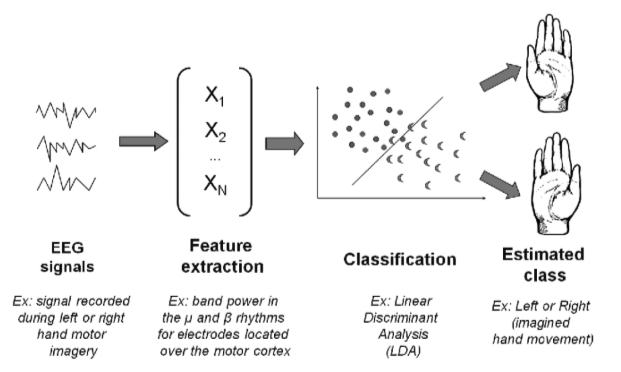
\includegraphics[width=0.8\textwidth]{eeg-pipeline.png}
    \caption{Ejemplo de las etapas por la que pasaría el procesamiento de una señal EEG \cite{eeg-tutorial}}.
	\label{fig:eeg-pipeline}
\end{figure}

En la figura \ref{fig:eeg-pipeline} se puede observar lo descripto anteriormente. Primero, se reciben las señales. Luego, se extraen las características. En este caso se trata de frecuencias asociadas a la corteza motora. Una vez que el vector de características fue creado, se envía al clasificador (en este caso análisis de discriminante lineal). Finalmente, el clasificador determina a que clase pertenece cada vector. En este ejemplo, se intento determinar si el usuario imaginó mover la mano derecha o la izquierda. 

Para medir la precisión del clasificador se arma una matriz de confusión. Esta, es una matriz de dos dimensiones en la cuál una dimensión representa los valores actuales y otra los valores predecidos. Por ejemplo, si utilizamos el ejemplo de ojos cerrados o abiertos, la matriz se armaría de la siguiente manera:

\[
\textrm{Mat} = \begin{blockarray}{ccc}
& A & C \\
\begin{block}{c(cc)}
  A & x & y \\
  C & w & z \\
\end{block}
\end{blockarray}
 \]
 
 , donde $ A $ representa el estado de ojos abiertos y $ C $, el de ojos cerrados. La primera dimensión representa el valor obtenido y la segunda el valor predecido. Por lo tanto, $Mat_{0,0}$ representa los positivos verdaderos ($TP$) (las veces que acertó el clasificador cuando el usuario tenía los ojos abiertos), $Mat_{0,1}$ representa los falsos negativos ($FN$) (valores que el clasificador clasificó como $C$ pero en realidad eran $A$), $Mat_{1,0}$ representa los falsos positivos ($FP$) (valores que el clasificador clasificó como $A$ pero en realidad eran $C$), y $Mat_{1,1}$ representa los verdaderos negativos ($TN$) (valores que el clasificador clasificó como $C$ y realmente eran $C$). Utilizando esta matriz se puede obtener la precisión, la cuál se define de la siguiente manera:
 
$$ ACC = \frac{TP + TN}{P + N} $$ 
, donde $P =$ total de casos positivos y $ N =$ total de casos negativos. O simplemente:

$$ ACC = \frac{Mat_{0,0} + Mat_{1,1}}{Mat_{0,0} + Mat_{0,1} + Mat_{1,0} + Mat_{1,1}} $$ 

Los valores cercanos a $0.5$ implican que el clasificador es malo y es azar. Cuantos más cercano $1$, mejor el clasificador.

Para determinar que parámetros de ajuste son los mejores para un modelo se puede utilizar el método de validación cruzada. Este consiste en subdividir un conjuntos de datos en dos subconjuntos, utilizar uno de ellos como datos de predicción y otro como de entrenamiento. Luego se validan los subconjuntos de entrenamiento contra el subconjunto de predicción y se toma la media. La validación cruzada más simple es el método de regresión. Aquí simplemente se dividen los datos de la muestra en dos particiones: una de entrenamiento y una de validación. Este método es rápido de computar pero el problema es que la evaluación puede depender en gran medida de como es la división entre datos de prueba y de entrenamiento. La varianza puede ser muy elevada. Una mejora a este método de validación cruzada de k iteraciones cruzadas. Este consiste en dividir los datos en $k$ subconjuntos y utilizar   $k$ veces regresión lineal. Cada iteración se elige un subconjunto como conjunto de validación y el resto son usados como conjuntos de entrenamiento. Es decir, se elige un único subconjunto de datos como conjunto de validación y los $k -1$ restantes, se utilizan como conjunto de entrenamiento. Luego se toma el promedio de todas las iteraciones \cite{cross-validation}.

\subsection{Salida}

Una vez que la señal fue procesada, la información obtenida está lista para ser utilizada. La salida puede ser, por ejemplo, una API de una librería que le permite a un usuario acceder a la información de forma amigable o una visualización en la computadora.

\section{Señales de Interés}

En la sección \ref{sec:biosignals} se introdujo el concepto de bioseñales y se mencionaron algunas de ellas. Este proyecto tiene foco en tres de ellas: 
electroencefalografía, electromiografía y pulsioximetría. En las siguientes secciones se brindará más información sobre las mismas.

\subsection{Electroencefalografía (EEG)}

La electroencefalografía detecta la actividad eléctrica de las neuronas, es decir, del cerebro. Con respecto a la clasificación, se trata de una señal permanente, ya que no debe ser inducida externamente, dinámica, ya que varía mucho en el tiempo, y eléctrica. Los dispositivos utilizados para realizar un eletctroencefalograma cuentan con una determinada cantidad de electrodos que miden el nivel de potencial eléctrico en $ \mu V$. Al utilizar uno de estos dispositivos, la señal digital que se obtiene es el nivel de potencial eléctrico en cada electrodo. Un electroencefalograma no sirve si no se le da alguna aplicación. Aquí aparece el concepto de Interfaz Cerebro-Computora (también conocido por sus silgas en inglés como BCI). "BCI es un método de comunicación basado en la actividad neuronal generada por el cerebro...El objetivo de BCI no es determinar la intensión de una persona espíando su actividad neuronal, sino que es proveer un nuevo canal de salida para el cerebro que requiere una adaptación de control voluntaria por parte del usuario"\cite{neural-eng}.

Al aplicar la Transformada de \emph{Fourier} a la señal EEG, se obtienen distintas frecuencias. En EEG, dichas frecuencias se dividen en cinco bandas:

\begin{itemize}
 \item \textbf{\emph{Alfa} ($\alpha$):} $ 8 \, Hz \leq f \leq 13 \, Hz$. Las ondas \emph{Alfa} se suprimen cuando los ojos se encuentran abiertos y hay estimulación visual presente. Cuando los ojos se encuentran cerrados, estas aumentan.
 \item \textbf{\emph{Beta} ($\beta$):} $ 13 \, Hz \leq f \leq 30 \, Hz$. Las ondas \emph{Beta} se asocian la concentración y aparecen como actividad de fondo en sujetos ansiosos. 
 \item \textbf{\emph{Delta} ($\delta$):} $ 0.5 \, Hz \leq f \leq 4 \, Hz$. Estas ondas aparecen en etapas de sueño profundo.
 \item \textbf{\emph{Theta} ($\theta$):} $ 4 \, Hz \leq f \leq 8 \, Hz$. Las ondas \emph{Theta} aparecen en las primeras etapas de sueño.
 \item \textbf{\emph{Gamma} ($\gamma$):} $ 30 \, Hz \leq f \leq 60 \, Hz $. Algunos expertos consideran los valores de $\beta > 30 \, Hz $ como una quinta banda. \cite{neural-eng}.
\end{itemize}

Como las frecuencias de interés abarcan hasta por los menos los $60 \, Hz$, se debe debe muestrar al menos a a $120 \, Hz$. Como se menciono anteriormente, muchas veces se utiliza una frecuencia de muestreo mayor y por lo general en EEG, se utiliza una frecuencia de muestreo superior a los $200 \, Hz$ \cite{neural-eng}.

\subsection{Electromiografía (EMG)}

La electromiografía consiste en registrar la actividad eléctrica producida por los músculos del cuerpo. La actividad eléctrica surge cuando una unidad motora es activada por el sistema nervioso del cuerpo: una unidad motora consiste en una motor neurona, y todas las fibras musculas a la que esta conectada.  Cuando se activa la unidad motora, se genera un voltaje (llamado MUAP, sus siglas en inglés) y se contraen los músculos.  Entonces, la señal EMG consiste en medir la suma de varios MUAPs de uno o mas músculos específicos. Con respecto a la clasificación, se trata de una señal permanente, ya que no debe ser inducida externamente, dinámica, ya que varía mucho en el tiempo, y eléctrica.

El rango de la amplitud de una señal EMG es de aproximadamente $0\ mV$ a $10\ mV$, y su frecuencia de $0\, Hz$ a $500\, Hz$.  Sin embargo, el rango dominante de energía de la señal es de los $50\, Hz$ a $150\, Hz$, el cual es el que se intenta medir en este proyecto. Por lo tanto, se debe muestrear al menos a $300 \, Hz$.

\subsection{Pulsioximetría (SpO2)}

La pulsioximetría permite determinar el porcentaje de sangre arterial saturado con oxígeno. Esta técnica no es invasiva y se basa en medir la absorción de luz roja e infraroja que pasa por el oído o dedo de una persona \cite{spo2-1}. Se basa medir una señal llamada \emph{Fotopletismografía}, la cual es una medición óptica del cambio de volumen de sangre en las arterias. Estas son obtenidas irradiando dos longitudes de onda de luz distintas a través del tejido. Existen dos formas de leer la oxigenación en sangre: transmisión y reflexión de la luz. En transmisión, se envían haces de luz utilizando una luz LED y se utiliza un fotodetector del otro lado que detecta estos haces. En cambio, en reflexión, se coloca un fotodetector del mismo lado que la luz led y se detecta la reflexión de la luz \cite{spo2-2}.  

El corazón bombea sangre a través de las arterias de forma continua. Este es conocido como el ciclo cardíaco. Este ciclo puede ser observado con un pulsioximetro ya que se generan variaciones de volumen en las arterias \cite{spo2-2}. En la figura \ref{fig:cardiac-cycle} se pueden observar los picos generados por el ciclo cardíaco. Dichos picos son utilizados para estimar el ritmo cardíaco. Esta señal es inducida, ya que se requiere de la utilización de una luz, dinámica, ya que varía de forma considerable en el tiempo, y, óptica. En este caso, la salida del transductor es binaria. Indica si ha habido un pico o no, por lo que no se genera ruido al digitalizarla.

\begin{figure}[H]
	\centering
    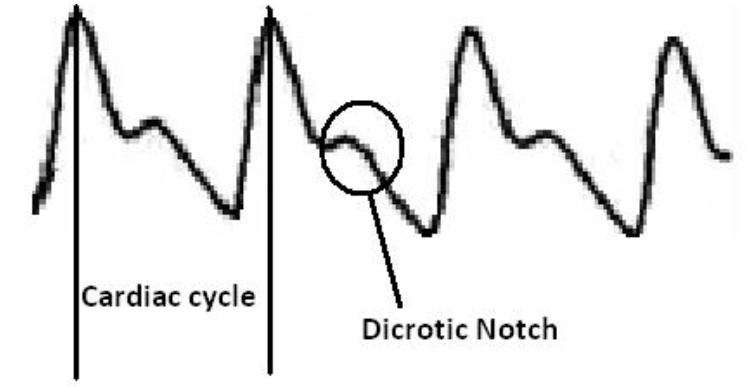
\includegraphics[width=0.8\textwidth]{cardiac-cycle.png}
    \caption{Ciclo cardíaco}.
	\label{fig:cardiac-cycle}
\end{figure}

Existen dos formas de calcular el ritmo cardíaco a partir de los picos:

\begin{itemize}
 \item \textbf{Promedio:} Se cuentan la cantidad de picos en un determinado tiempo y luego se utiliza la regla de tres simple. El problema es que este método no permite observar cambios en el tiempo y por lo tanto no representa verdaderamente la respuesta al ejercicio, el estrés y el ambiente.
 \item \textbf{Latido a latido:} Se mide el tiempo ($T$) entre dos picos consecutivos y luego se calcula usando la fórmula $60/T$ \cite{spo2-1}.
\end{itemize}

Se pueden combinar estas dos metodologías y promediar los últimos cuatro o seis resultados obtenidos \cite{spo2-1}.



\chapter{Implementación}
En este capítulo se hablará sobre la implementación realizada. Primero, se mencionarán las señales elegidas y se dará una explicación de por qué se tomo esta decisión. Luego, se introducirá el \emph{hardware} utilizado. Después, se explicará de que manera se procesaron las distintas señales, desde la obtención de las mismas hasta las características y clasificadores utilizados. Finalmente, se hablará de los universos 3D interactivos desarrollados. Los universos 3D fueron desarrollados en el lenguaje \emph{C\#} en \emph{Unity}.

\section{Elección de las señales}

Primero se tuvo que elegir que señales se iban a procesar. Para llevar a cabo esta elección, se tuvieron en cuenta los siguientes criterios:

\begin{itemize}
\item \textbf{Practicidad:} Se buscó que el sensor requerido para obtener la señal no sea invasivo y que sea fácil de utilizar por personas no técnicas.
\item \textbf{Uso en universos interactivos:} Que se le pueda dar un uso coherente en universos interactivos. Incluye el dinamismo de la señal ya que las señales casi estáticas no muestran una variabilidad suficiente para ser detectada en un período de tiempo de corta duración.
\item \textbf{Tiempo de procesamiento} El tiempo de procesamiento de las señales obtenidas debía ser aceptable para uso en tiempo real.
\item \textbf{Precio y disponibilidad} Se buscó que existan dispositivos disponibles en el mercado y a precios accesibles.
\end{itemize}

Utilizando estos criterios, se eligieron las siguientes señales: \acrshort{eeg}, \acrshort{emg} y \acrshort{spo2}. Todas ellas cumplen con la condición de ser prácticas y no invasivas, lo suficientemente dinámicas para que sean aplicables en nuestro estudio, que el tiempo de procesado sea apto para el tiempo real, y que los sensores fueron accesibles y comerciales como para poder probarlos e implementarlos.

\subsection{\acrshort{eeg}}

Existen sensores para capturar este tipo de señal que son no invasivos. Simplemente se utilizan electrodos superficiales, que se sitúan sobre la piel, en diversas partes de la cabeza. Además, el cerebro refleja mucho el estado del usuario por lo que la información extraída de él resulta muy útil e interesante para utilizar en universos interactivos. Al investigar, se descubrió que existen diversos dispositivos (no muy costosos) que tienen una frecuencia de muestreo superior a los $200 \, Hz$ y como se mencionó anteriormente, las frecuencias de interés llegan hasta $60 \, Hz$ , lo cual  permite su uso en tiempo real. El hecho de que la frecuencia de muestreo no sea muy elevada permite que se puedan procesar los datos rápidamente. Si la frecuencia fuese muy elevada, tal vez no se podrían procesar en tiempo real y habría una latencia muy elevada. A su vez, la colocación de dicho sensor es fácil. Por lo general se coloca una banda o casco en la cabeza, por lo cuál puede ser utilizado por personas no técnicas.

\subsection{\acrshort{emg}}

Para capturar esta señal, existen electrodos invasivos y no invasivos por lo cual cumple con el primer criterio. Las frecuencias de interés son entre $0 \, Hz $ y $150 Hz$ y existen diversos dispositivos con frecuencias de muestreo mayores a $300 \, Hz$ por lo cual se puede utilizar en tiempo real. Además, con este tipo de dispositivos, se puede medir la fuerza realizada por los músculos. Resulta muy interesante poder medir y detectar cambios en la fuerza realizada por los músculos y utilizar esta información para controlar acciones en universos interactivos. Existen también otro tipo de electrodos de monitoreo \acrshort{emg}: los intramusculares, que van insertados dentro del musculo del sujeto. Este tipo de electrodos no fueron utilizados en este proyecto ya que son muy invasivos, y muy imprácticos dentro del contexto de diseñar un sistema que pueda ser utilizado fácilmente por cualquier persona sin conocimientos técnicos del área.

\subsection{\acrshort{spo2}}

La \gls{spo2} no es una técnica invasiva. Como se menciono anteriormente, utiliza luces y fotodetectores. El ritmo cardíaco resulta de mucho interés para ser utilizado en universos interactivos ya que su estado puede reflejar que tan nervioso se encuentra el usuario y utilizar dicha información para alterar el estado de la simulación. A su vez, los picos se miden en tiempo real. Su utilización es tan simple como colocar el pulsioxímetro en un dedo.

Se decidió utilizar un pulsioxímetro en lugar de un dispostivo \acrshort{ekg} ya que es más práctico. El \emph{Olimex SHIELD-EKG-EMG} resultaba muy incómodo de utilizar debido a que uno de los electrodos debía colocarse en una pierna y otro en un brazo, lo que hubiese ocasionado dificultad para operar una computadora mientras se utilizaba. Si bien un dispositivo EKG es más preciso que un pulsioxímetro, estudios han demostrado que la estimación realizada por un pulsioxímetro es muy precisa cuando el ritmo cardíaco se encuentra por debajo del $89\% $ de su máximo \cite{spo2-accuracy}. Como el usuario se encuentra sentado en una computadora, jamás alcanzará dichos valores.

Además, como ya se contaba con dos señales eléctricas permanentes, se buscó una señal con otra clasificación.

\section{Hardware}

Para la elección de los dispositivos de \emph{hardware} se tuvieron en cuenta los criterios antes mencionados buscando un compromiso entre costo y fiabilidad así como también se tuvo en cuenta su facilidad de uso.

\subsection{\acrshort{eeg}}

En el caso de \acrshort{eeg}, se decidió utilizar el \emph{Muse Brainsensing Headband}. Este dispositivo cuenta cuenta con siete electrodos y diversas funcionalidades. En la figura \ref{fig:muse-electrodes} se puede observar la configuración del dispositivo. Cuenta con tres electrodos de referencia sobre la frente, dos electrodos frontales y dos electrodos en las orejas. Los electrodos de referencia se utilizan para medir el nivel de potencial eléctrico. Es decir, el potencial de los restantes electrodos, se mide en base a los electrodos de referencia.

\begin{figure}[H]
	\centering
    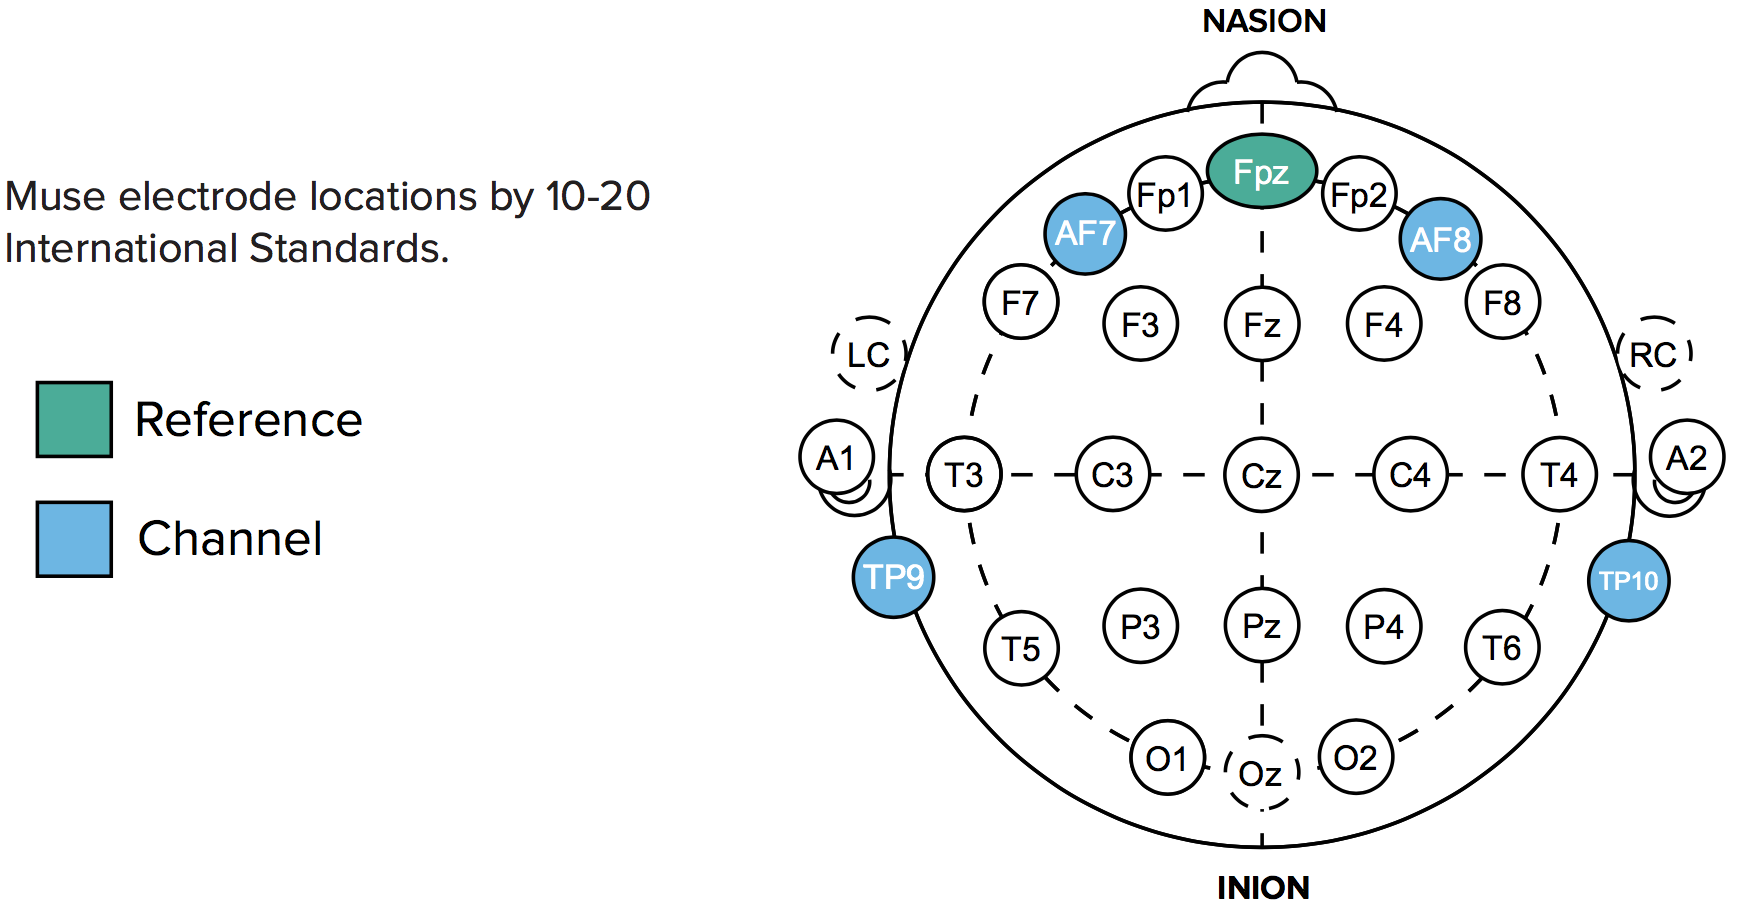
\includegraphics[width=0.8\textwidth]{muse-electrodes.png}
    \caption{Diagrama de la ubicación de los electrodos en el \emph{Muse Brainsensing Headband}. AF7 y AF8 son los electrodos frontales, TP9 y TP10 los electrodos en las orejas y Fpz representa los tres electrodos de referencia \cite{muse-hardware}.}
	\label{fig:muse-electrodes}
\end{figure}

En la figura \ref{fig:eeg-raw} se puede observar las señal \acrshort{eeg} bruta de los cuatro electrodos del sensor.

\begin{figure}[H]
	\centering
    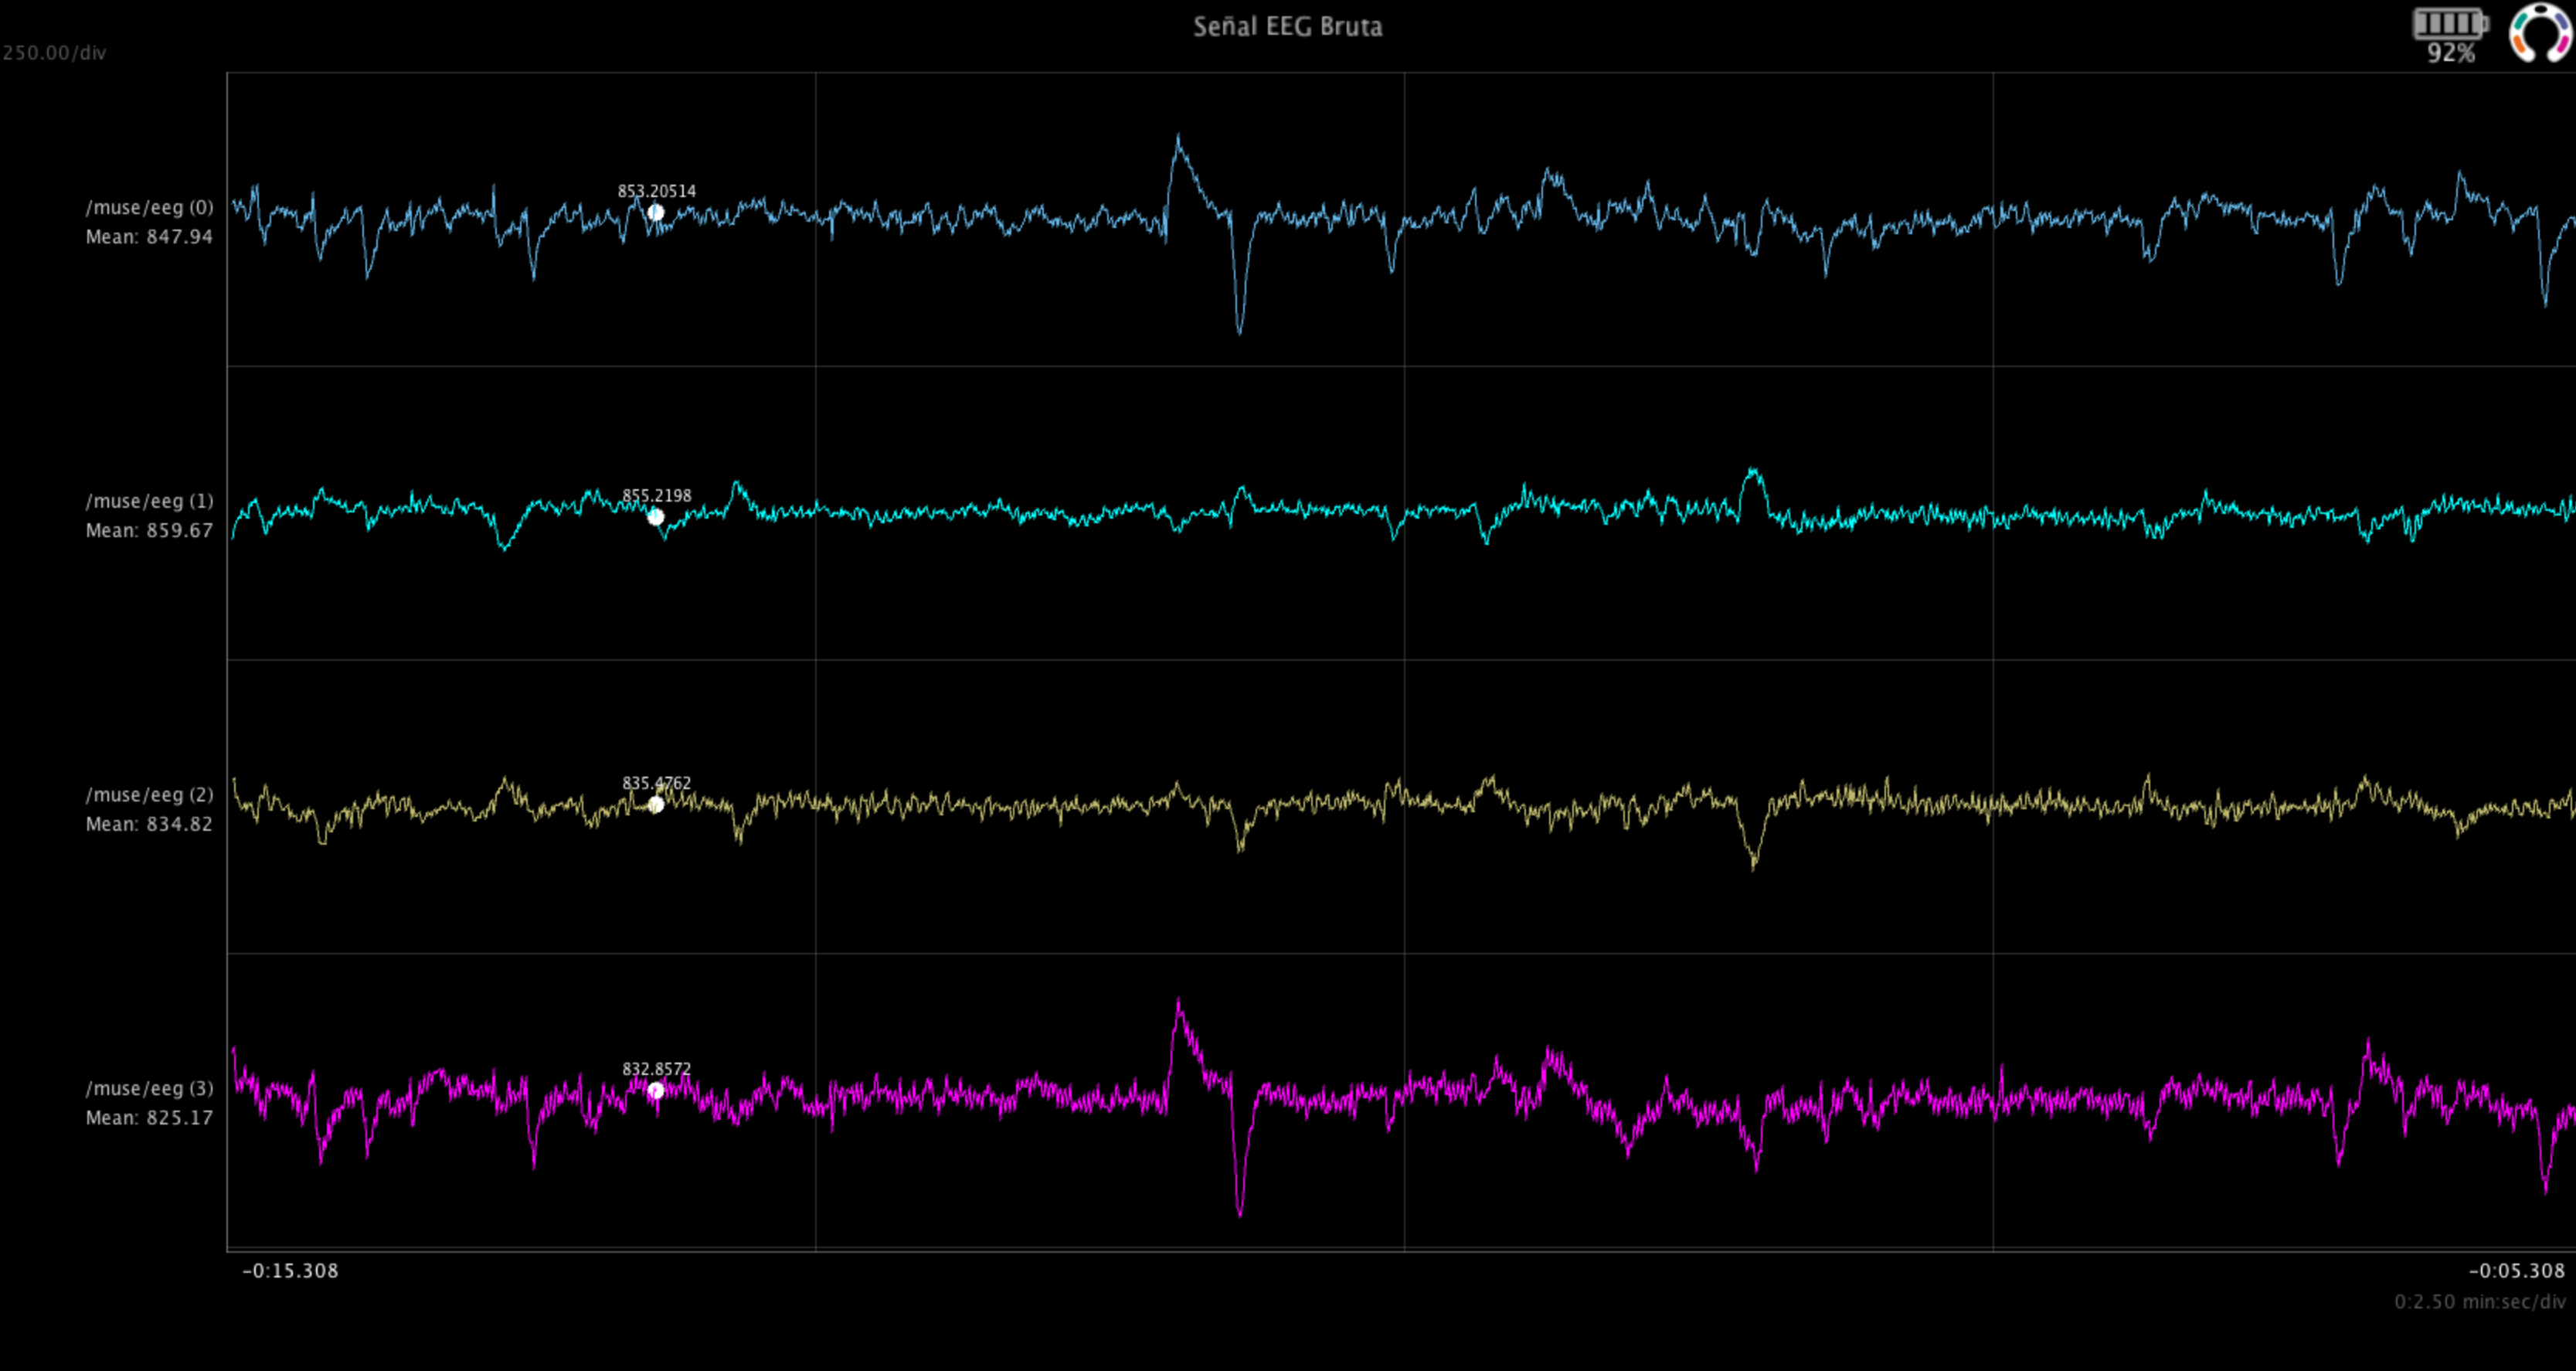
\includegraphics[width=0.8\textwidth]{eeg-raw.png}
    \caption{Señal EEG bruta de cada uno de los electrodos obtenido utilizando la aplicación \emph{MuseLab}.}
	\label{fig:eeg-raw}
\end{figure}

El dispositivo tiene una frecuencia de muestreo de $ 256 \, Hz$. Además cuenta con acelerómetro y giroscopio lo que permite medir la orientación del usuario. También cuenta con un puerto micro USB y \emph{bluetooth}. Permite acceder a la información bruta de cada electrodo por lo que se obtienen cinco valores. Cuatro de de los electrodos frontales y de las orejas, y el restante se obtiene de los tres electrodos de referencia. También brinda algunas facilidades como realizar la Transformada de \emph{Fourier},  calcular la potencia de las bandas ($\alpha$, $\beta$, $\delta$, $\theta$ y $\gamma$), entre otros.

Para los desarrolladores, cuenta con \acrshort{sdk} para \emph{Windows} y \emph{Unity} y cuenta con aplicaciones multiplataforma para poder acceder a los datos. Una forma de acceder a los datos es a través de \gls{osc}. \acrshort{osc} es un protocolo que corre sobre \acrshort{udp} y permite el \emph{stream} continuo de datos.

\subsection{\acrshort{emg}} \label{emg-hardware}

Para la lectura de señales EMG, se optó por utilizar la plataforma Arduino, con un modulo adicional diseñado para la captura de señales \acrshort{emg} y \acrshort{ekg}.  Arduino es una plataforma que consiste en varios micro controladores de diseño abierto (\emph{Open Source Hardware}), y un software que permite programarlos de forma fácil y rápida utilizando el lenguaje de progamación \emph{C++}. Los programas que son compilados e instalados en el \emph{Arduino} son conocidos como \emph{sketches}.

El modelo de Arduino elegido fue el \emph{Arduino Mega 2560}, que cuenta con un procesador que opera a $16\, MHz$, y cuenta con $256 Kb$ de memoria para programas, lo cual prácticamente permite trabajar sin restricciones de memoria en mente. A su vez, el modulo adicional elegido fue el \emph{Olimex SHIELD-EKG-EMG}, que trae electrodos superficiales que pueden ser ubicados sobre la piel del musculo que se intenta monitorear.  Los electrodos cuentan con tres terminales, marcadas con las letras $L$ (izquierda), $R$ (derecha) y $D$ (referencia) (figura \ref{fig:emg-electrodes}). Los valores leídos por los electrodos son procesados por tres filtros: dos filtros pasa altos de $16\, Hz$, y un filtro \emph{Bessel} de $40\, Hz$, que similar a un filtro \emph{Gaussiano}.

\begin{figure}[H]
	\centering
    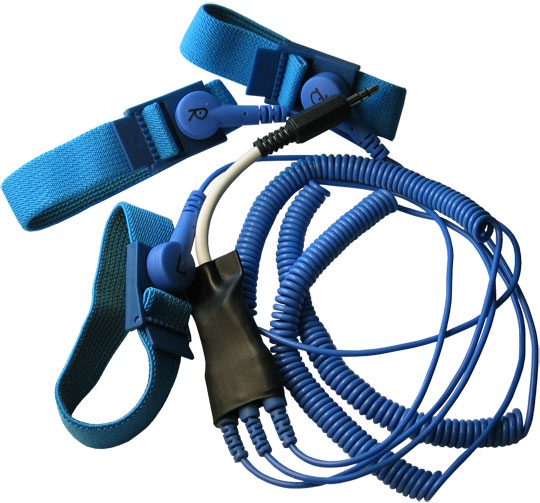
\includegraphics[width=0.5\textwidth]{electrodes.jpg}
    \caption{Electrodos superficiales para el modulo \emph{Olimex SHIELD-EKG-EMG} \cite{emg-electrodes}.}
	\label{fig:emg-electrodes}
\end{figure}

Para poder leer las señales EMG, se debe preparar el sistema de monitoreo.  Primero, se debe montar el modulo EMG sobre el micro controlador \emph{Arduino}.  El \emph{Arduino} debe tener instalado un \emph{sketch} específico, detallado en la sección \ref{sec:emg-signal-processing}. Luego, las terminales $L$ y $R$ se deben posicionar sobre la piel del musculo a monitorear, y la terminal $D$ debe ser posicionada sobre una superficie del cuerpo a utilizar como referencia, que preferiblemente no contenga musculos, o tenga musculos no relacionados a los de las otras dos terminales (a este circuito se le llama \emph{Driven Right Leg Circuit} en inglés). En este proyecto, se opto por medir la actividad muscular de un brazo, junto a la mano, al formar un puño cerrado apretado. Por lo tanto, los electrodos fueron colocados sobre el músculo flexor común superficial de los dedos, que se encuentra sobre la cara anterior de antebrazo\cite{emg-signals-wrist}. Una vez realizados los pasos anteriores, se puede proceder a conectar el micro controlador a la computadora vía un cable USB 2.0.

Para comprobar el correcto funcionamiento del dispositivo, se utilizó un software llamado \emph{ElectricGuru}, recomendado por los fabricantes del módulo \acrshort{eeg}. Si el sistema de monitoreo fue preparado correctamente, el software debería mostrar una pantalla similar a la siguiente:

\begin{figure}[H]
	\centering
    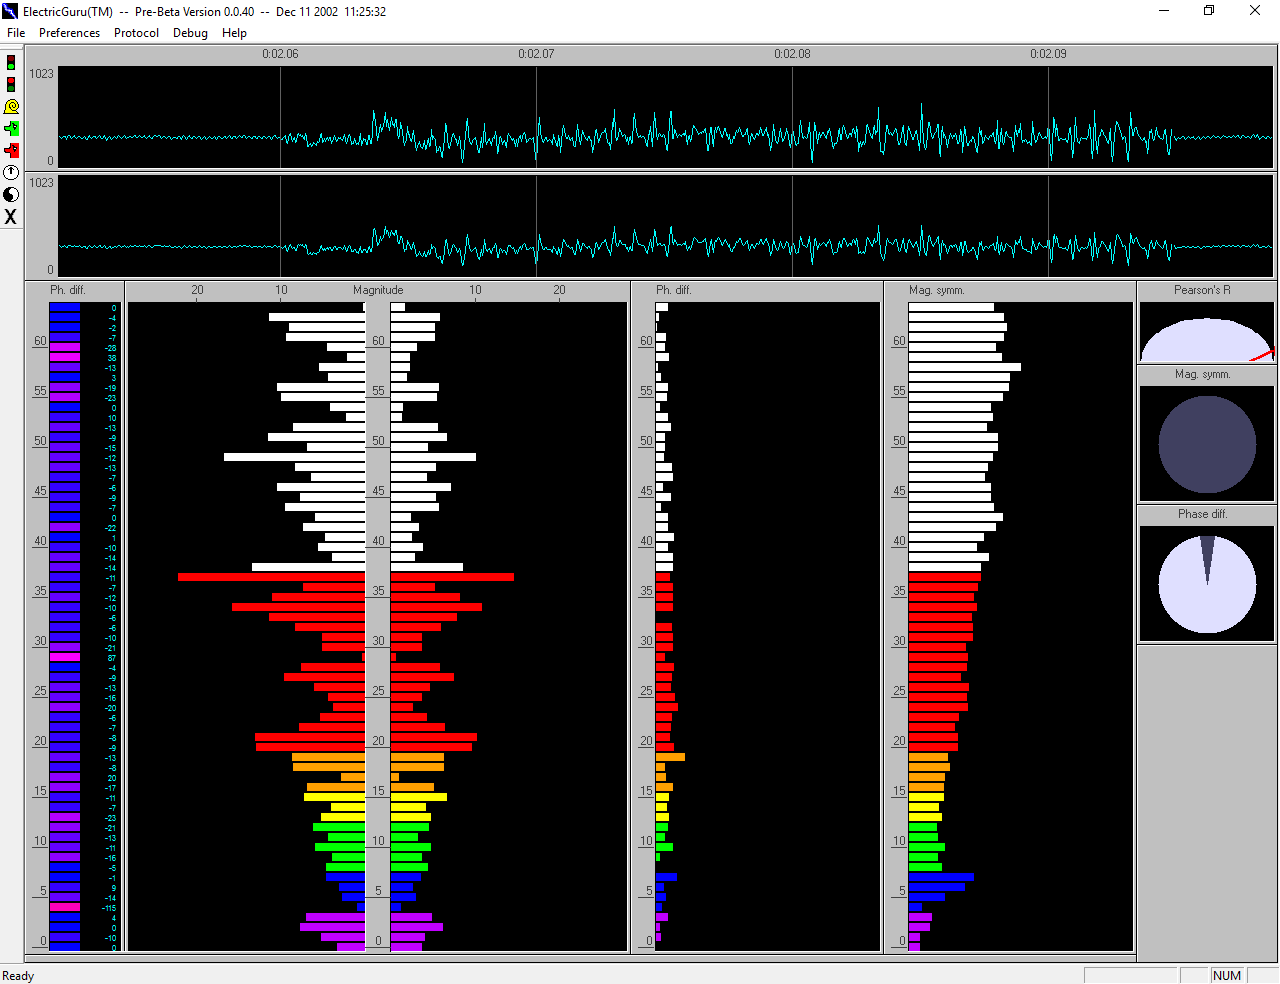
\includegraphics[width=0.8\textwidth]{electricguru.png}
    \caption{Pantalla principal de \emph{ElectricGuru}, leyendo señales \acrshort{emg}.}
	\label{fig:emg-electricguru}
\end{figure}

\subsection{\acrshort{spo2}}

Para medir el ritmo cardíaco se decidió utilizar el dispositivo \emph{CMS50D+ Contec Pulse Oximeter}. Éste es un pulsioxímetro de transmisión de alta precisión, fácil de utilizar y de bajo consumo. Dicho dispositivo utiliza el puerto serie para enviar datos utilizando un formato propietario. Los datos más relevantes que envía el sensor son:

\begin{itemize}
\item \textbf{Picos:}  Indica si hubo un pico.
\item \textbf{Ritmo cardíaco:} Estimado utilizando una ventana de 30 segundos.
\item \textbf{Oxígeno:} Porcentaje de oxígeno.
\end{itemize} 

El dispositivo se conecta a la computadora con un cable USB 2.0 que internamente convierte de serie a USB. Se debe contar con un controlador de puerto serie en la computadora que permita su lectura. La frecuencia de muestreo es de $256 \, Hz$. El margen de error del dispositivo utilizado es de $\pm2\%$ para la medición de \acrshort{spo2} y ritmo cardíaco. Éste margen de error pequeño se debe a que el \emph{CMS50D+} es un dispositivo médico, con lo que se necesita que sea lo más preciso posible.

\section{Obtención y Procesamiento de Señales}

Para cada uno de los sensores se evaluaron y aplicaron distintas alternativas sobre como procesar la señal. El objetivo al procesar las señales fue que dicho procesamiento sea lo suficientemente preciso como para poder ser utilizado en tiempo real en universos 3D.

\subsection{\acrshort{eeg}} \label{sec:eeg-signal-processing}

Para leer la señal se decidió utilizar \emph{OSC}. Se tomó esta decisión ya que al momento de iniciar el proyecto, el \acrshort{sdk} para Windows se encontraba en estado beta por lo que no era confiable. Además implicaba un desarrollo en el lenguaje \emph{C} mientras que el desarrollo se encontraba en \emph{C\#} y, como solo se encontraba disponible para \emph{Windows}, no permitía que el proyecto sea multiplataforma. Tampoco se utilizó el \acrshort{sdk} para \emph{Unity}, ya que este era únicamente para dispositivos móviles.

Una gran desventaja de este dispositivo, es que no cuenta con soporte para la aplicación \emph{MuseIO}, que permite obtener paquetes \acrshort{osc} a través de la computadora. Por este motivo, se terminó utilizando una aplicación móvil llamada \emph{Muse Monitor}, que nos permitió conectar el dispositivo al teléfono celular y desde allí enviar los paquetes \acrshort{osc} hacia la computadora. En un principio se pensó que la latencia podría ser un problema ya que cada paquete debe realizar dos trayectos, primero desde el dispositivo hacia el teléfono celular y luego hacia la computadora, pero esto no fue un problema ya que el flujo de datos no era masivo y los paquetes no eran de gran tamaño.

Inicialmente, se utilizó un \emph{framework} para procesar los paquetes \acrshort{osc} pero este no resultó ser fiable. Se buscaron alternativas pero no hubo ninguna que cumpla con los estándares del equipo. Por este motivo, se desarrollo un procesador de paquetes \acrshort{osc} propio basado en otras implementaciones. Esto implicó leer el estándar, comprender como funciona e implementarlo.
 
 Los estados que se buscaron detectar fueron ojos abiertos (A) y ojos cerrados (C). Por este motivo, la información que se necesitaba eran las ondas $\alpha$. Como se mencionó anteriormente, el dispositivo \emph{Muse} permitía acceder a la potencia de las ondas $\alpha$. Para obtener dichas ondas el dispositivo sigue el siguiente procedimiento:
 
 \begin{enumerate}
 \item Obtener una ventana de $25$ muestras (pues envía $10$ muestras por segundo y el sensor obtiene $256$ muestras por segundo) y aplicar la función de ventana $Hann$.
 \item Obtener la Transformada de \emph{Fourier} de la ventana.
 \item Aplicar un filtro pasa banda para utilizar únicamente las frecuencias de interés ( $ 8 \, Hz \leq f \leq 13 \, Hz$).
 \item Realizar la \acrshort{psd} sobre esos valores. A diferencia de solo integrar, el dispositivo aplica $log_{10}$  a cada valor antes de realizar la integral.
 \end{enumerate}

El vector de características se confeccionó utilizando dos valores de \emph{Alpha} consecutivos, es decir, de la siguiente manera:

\[
  \vec{v}^{\, }=
  \left[ {\begin{array}{cc}
   \alpha_{i}  & \alpha_{i + 1}  \     \end{array} } \right]
\]

En la etapa de entrenamiento se le asignaba un estado a cada uno de estos vectores. Se le indicaba a al usuario en que momento abrir y cerrar los ojos y se registraba el estado para dichos valores. La precisión obtenida con este método fue en promedio de aproximadamente un $65\%$. Esto se debe a que aún cuando el usuario se encontraba con los ojos abiertos, \emph{Alfa} alcanzaban valores tan altos como cuando el usuario se encontraba con los ojos cerrados debido a posibles ruidos del sensor y a el hecho de que las bioseñales varían mucho. Se podía observar que el clasificador era muy preciso en detectar ojos cerrados pero muy impreciso en detectar ojos abiertos. La precisión en ojos cerrados era de un $99\%$ y en ojos abiertos de un $25\%$.

Para intentar mejorar la precisión, se decidió aumentar el tamaño de la ventana con la expectativa de que al tener una mayor cantidad de valores, los picos anómalos que se generaban cuando el usuario estaba con los ojos abiertos, se redujeran ya que al contar con más muestras es probable que se obtenga una mayor cantidad de valores que corresponden al estado de ojos abiertos. Se podría decir que los picos anómalos se promedian al tener una mayor cantidad valores normales. Cuando se trabaja con bioseñales, cuantos más datos se tomen, más robusta será la clasificación. El problema es que para tomar más datos se necesita más tiempo. Entonces, aquí aparece un compromiso entre robustez y latencia. Como en este proyecto la utilización fue en tiempo real, hubo que considerar seriamente este compromiso. A su vez, cuanto mayor sea la frecuencia de muestreo, mayor es el espacio entre frecuencias y como consecuencia se pueden representar con más granularidad dichas frecuencias. El dispositivo utiliza una frecuencia de $10 \, Hz$ para los valores de potencia de \emph{Alfa} y se necesitaba una frecuencia mayor, por lo que se decidió calcular dicha potencia utilizando los datos brutos. El dispositivo envía un arreglo de cinco elementos. Como se mencionó anteriormente, el quinto valor es de referencia por lo que se ignora en el procesamiento. El procedimiento implementado fue el siguiente:

 \begin{enumerate}
 \item Obtener una ventana $256$ muestras, es decir, un segundo.
 \item Obtener la Transformada de \emph{Fourier} de la ventana.
 \item Quedarse únicamente con las frecuencias $8 \, Hz-13 \, Hz$.
 \item Realizar la \acrshort{psd} sobre esos valores.
 \end{enumerate}
 
Este procedimiento se aplica por cada uno de los cuatro electrodos. Por lo que cada segundo, se cuenta con cuatro valores. El vector de características se forma con estos cuatro valores de la siguiente manera:
 
\[
  \vec{v}^{\, }=
  \left[ {\begin{array}{cccc}
   \alpha_{AF7}  & \alpha_{AF8} & \alpha_{TP9} & \alpha_{TP10}  \     \end{array} } \right]
\] 

Con este vector de características, se alcanzó una precisión de hasta un $ 90 \%$. Esto se debe a que, si bien empeoro la precisión de detectar ojos cerrados, incrementó notablemente la de ojos abiertos.
 
Se probó aplicar un filtro \emph{Gaussiano} a la señal bruta pero se obtuvieron exactamente los mismos resultados. Ya que en la documentación no se especifica que tipos de filtros se aplican, la ausencia de ruido \emph{Gaussiano} podría ser explicada por dos motivos: o el sensor ya cuenta con filtros que reducen el ruido sensible a filtrados \emph{Gaussianos}, o bien que la etapa de cuantificación es lo suficientemente precisa como para no introducir ruido blanco (o una combinación ambos). A su vez, se implementó un \emph{detrending} lineal de la señal pero tampoco se notaron diferencias sustanciales. El método de \emph{detrending} calculaba la media de todas las muestras obtenidas del sensor durante un cierto periodo de tiempo, y luego le restaba ésta a todas las muestras leídas más adelante. Al haber alcanzado el nivel de precisión que se buscaba, se decidió concluir con el procesamiento de la señal en este punto. Es decir, no se aplicaron filtros de pasa-banda ni funciones de ventana porque no se consideró necesario.
 
En la etapa de entrenamiento, en lugar de tomar todos los valores, se ignoran los valores de transición. Cuando se le indica al usuario que abra o cierre los ojos, se descartan dos segundos antes y después de la transición de estados. Esto se debe a que los valores que corresponden a la transición no son significativos. Los que realmente importan son cuando se está en un estado u otro.
 
\subsection{\acrshort{emg}} \label{sec:emg-signal-processing}

Una vez preparado el sistema de monitoreo EMG descripto en la seccion \ref{emg-hardware}, se puede comenzar a leer los datos. Los micro controladores \emph{Arduino} permiten comunicarse a una computadora mediante un puerto de serie que es establecido a traves de la conexión USB.  Para poder leer del puerto de serie desde el sistema operativo, es necesario conocer los parametros de la conexión (velocidad, paridad, cantidad de bits de información, etc.), y el nombre del puerto de serie. Los valores utilizados fueron los predeterminados utilizados en el programa de ejemplo referenciado en el manual del módulo \acrshort{emg} \cite{olimex-manual}.

En la version inicial del \emph{sketch}, la frecuencia de muestreo toma el valor de $256\, Hz$. Por el teorema de muestreo de Nyquist-Shannon, esto quiere decir que dadas estas muestras, solo es posible reconstruir señales con frecuencias iguales o inferiores a $128\, Hz$. Teniendo esto en mente, el procedimiento llevado a cabo para leer los datos de \acrshort{emg} fueron los siguientes:

 \begin{enumerate}
 \item Obtener una ventana $128$ muestras, es decir, medio segundo.
 \item Obtener la Transformada de \emph{Fourier} de la ventana.
 \item Quedarse únicamente con las frecuencias en el rango de $50 \, Hz-128 \, Hz$. Las frecuencias en el rango de $128 \, Hz-150 \, Hz$ no son capturadas.
 \item Separar el rango de frecuencias resultante en dos mitades: $50 \, Hz-89 \, Hz$ y $90 \, Hz-128 \, Hz$.
 \item Realizar la \acrshort{psd} sobre ambas mitades por separado.
 \end{enumerate}

Luego de haber realizado los pasos mencionados, el resultado son dos valores numéricos representativos de la intensidad de la señal recibida.  Utilizando estos dos valores, se construyo el vector de características de la señal \acrshort{emg}. Con este vector, se lograron precisiones de predicción muy altas (superiores a $ 95 \%$), utilizando tiempos de entrenamiento de alrededor de $5$ minutos.

Se implementó la técnica de \emph{detrending} de muestras, pero al no encontrar mejoras significativas en precision de los resultados, se decidió no utilizarlo para reducir la cantidad de código en el proyecto. También, no se aplicó un filtro de \emph{Gauss} ya que la precisión alcanzada fue lo suficientemente alta para las necesidades de este proyecto (como se explica en la sección \ref{sec:emg-results}). Además, como se mencionó anteriormente, el módulo \acrshort{emg} ya utilizaba filtros, por lo que la señal no tenía cantidades significativas de ruido.

Para el entrenamiento, el procedimiento fue simple. Primero, se preparo el sistema de monitoreo \acrshort{emg}, y se colocaron los electrodos sobre la piel del los músculos mencionados en la sección \ref{emg-hardware}. Luego, con el brazo y mano relajados, se comenzó a entrenar un clasificador con las muestras leídas y procesadas. A continuación se procedió a tensar el brazo y cerrar la mano con fuerza, con tal de generar una diferencia de potencial significativa, en intervalos intermitentes de alrededor de $15$ segundos. Durante todo el proceso, se le informa al clasificador a que categoría pertenece cada dato ingresado (musculo tensionado o relajado).

Luego de experimentar con el valor preestablecido de $256\,Hz$ para la frecuencia de muestreo, se decidió intentar con una frecuencia mas alta, $512\,Hz$. La primera ventaja que esto trae es que, si se sigue tomando una ventana de $128$ muestras para la generación de un vector de características, el tiempo transcurrido entre cada valor generado pasa de ser de $0,5$ segundos a $0,25$ segundos. Desde un punto de vista de interacción de usuario, esto quiere decir que la simulación puede reaccionar mas rápido ante cambios de tension de musculo, lo cual permite que la experiencia sea mas fluida y tenga un mejor tiempo de respuesta. La segunda ventaja que trajo el cambio de frecuencia de muestreo es que, por el teorema de Nyquist-Shannon mencionado anteriormente, el rango de frecuencias de $50 \, Hz-150 \, Hz$ deseado ahora pudo ser analizado en su enteridad. Al aumentar la frecuencia de muestreo, también aumentó la cantidad de datos transmitidos desde el micro controlador hasta la computadora, por lo que hubo que aumentar la velocidad de transmisión del puerto de serie para compensar.

Al igual que en \acrshort{eeg}, al transicionar de un estado de tension de musculo a otro, se ignora cierta cantidad de muestras luego del momento de la transición, ya que solo son de interés los datos leídos al mantener un estado de tension constante. 

Al realizar los experimentos, se notó que ocasionalmente los datos leídos contenían grandes cantidades de ruido, por lo que eran prácticamente inutilizables. El problema encontrado fue que el sujeto conectado al modulo \acrshort{emg} no estaba eléctricamente aislado al suelo, lo cual introducía ruido a los valores leídos. El problema fue resuelto asegurándose de que el sujeto utilizara calzado con suficiente aislación eléctrica, como por ejemplo botas o zapatillas deportivas.

\subsection{\acrshort{spo2}} \label{sec:spo2-signal-processing}

Como se mencionó anteriormente, el dispositivo elegido utilizaba un formato propietario. Por este motivo, no se podía obtener una correcta lectura de los datos. La única forma de obtener los datos era realizando ingeniería inversa sobre el protocolo utilizado. Se investigó y se encontró cómo era la estructura interna de cada paquete recibido. Una vez que se podían leer paquetes, estos debían ser procesados. El ritmo cardíaco calculado por el sensor utiliza una ventana de 30 segundos. Esta duración era inaceptable para utilizar en tiempo real ya que reflejaba el ritmo cardíaco calculado sobre los 30 segundos anteriores, la cual es una duración de tiempo demasiado extensa en una aplicación interactiva. Por ésta razón, se decidió calcular el ritmo cardíaco utilizando los picos del ciclo cardíaco, utilizando una ventana más pequeña.

El dispositivo obtiene $256$ muestras por segundo, pero el ritmo cardíaco de una persona en reposo se encuentra entre los $60$ - $100$ \acrshort{bpm}. Por lo tanto, para cada latido, hay múltiples paquetes consecutivos indicando que hubo un pico. Para evitar estimar incorrectamente, se estableció un tiempo mínimo $t$ segundos que debía transcurrir entre picos. Entonces, si se recibía un paquete indicando un pico luego de menos de $t$ segundos del anterior, simplemente se lo considero como parte del mismo pico del ciclo cardíaco.

En una primera aproximación, se utilizó una ventana de $10$ segundos y se calculaba el ritmo cardíaco utilizando la técnica de promedio. Dicha técnica no resultó efectiva ya que el ritmo cardíaco contaba con grandes fluctuaciones lo que causaba que sea inutilizable en tiempo real. Luego, se empezó a utilizar la técnica de medir el tiempo entre latidos y realizar el promedio de los últimos nueve valores. Esta técnica resultó efectiva indicando un ritmo cardíaco estable y suficientemente preciso. Se comparó con el valor de ritmo cardíaco obtenido por el sensor para determinar si era preciso. A su vez se comparó con lo medido por un \emph{Apple Watch}.

Con este sensor simplemente se buscaba observar si el ritmo cardíaco superaba un umbral por lo que no requirió reconocimiento de patrones.

\section{Desarrollo de Universos 3D Interactivos} \label{sec:unity-net}

Para el desarrollo de universos 3D se decidió utilizar el motor gráfico para videojuegos \emph{Unity 3D}, junto al lenguaje de programación \emph{C\#}. Se tomó esta decisión por diversas razones. En primer lugar, el motor \emph{Unity} fue diseñado para ser multiplataforma: puede ser utilizado para crear juegos y/o aplicaciones para \emph{macOS}, \emph{Windows}, \emph{GNU/Linux}, \emph{iOS} y \emph{Android}, entre otras. En segundo lugar, también se eligió por su flexibilidad y robustez: es utilizado por varios estudios profesionales de videojuegos, y también por una gran cantidad de usuarios independientes, por lo que cuenta con una gran comunidad de creadores.

El motor gráfico \emph{Unity} puede ser utilizado/extendido con distintos lenguajes de programación, siendo \emph{C\#} uno de ellos. \emph{C\#} es un lenguaje creado por \emph{Microsoft} como parte de la plataforma \emph{.NET}.  La plataforma \emph{.NET} es similar a la plataforma \emph{Java}: su diseño esta centrado en una maquina virtual llamada \gls{cil}, que ejecuta código de tipo \acrshort{cil}, que es obtenido al compilar código \emph{C\#}:

\begin{figure}[H]
	\centering
    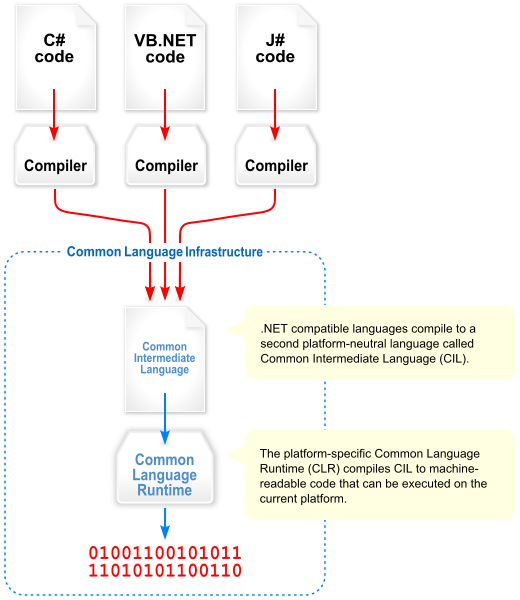
\includegraphics[width=0.5\textwidth]{clr.png}
    \caption{Diagrama de la arquitectura de la plataforma \emph{.NET}.}
	\label{fig:net-clr}
\end{figure}

Aunque \emph{Unity} permite el uso de \emph{C\#} para su extensión, no utiliza la máquina virtual \emph{CLR} para su funcionamiento. En cambio, utiliza una herramienta propietaria llamada \acrshort{il2cpp}, que traduce código \acrshort{cil} a código \emph{C++}. Al ser \emph{C++} un lenguaje extremadamente popular y difundido, éste puede ser luego compilado a cualquier código nativo que sea necesario para cada plataforma individual. De ésta forma, \emph{Unity} permite utilizar código compilado a \acrshort{cil} en cualquier plataforma, sin utilizar una maquina virtual:

\begin{figure}[H]
	\centering
    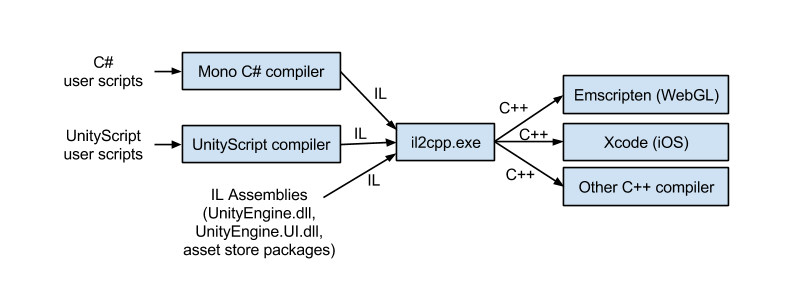
\includegraphics[width=1\textwidth]{unity.png}
    \caption{Diagrama de la arquitectura de compilación para el motor gráfico \emph{Unity}. Las siglas \emph{IL} equivalen a el \acrshort{cil} del diagrama \ref{fig:net-clr} \cite{il2cpp}.}
	\label{fig:unity}
\end{figure}

Como se muestra en la figura \ref{fig:unity}, cualquier archivo conteniendo código en formato \acrshort{cil} puede ser utilizado como parte del juego o aplicación. Como consecuencia de ésto, se pudieron utilizar librerías diseñadas para la plataforma \emph{.NET} como parte del desarrollo del proyecto. Una de las librerías utilizadas fue \emph{Accord.NET} (versión $3\text{.}3\text{.}0$), que cuenta con varios módulos relacionados al aprendizaje automático y a la matemática\cite{accord-net}. También, se utilizó la librería estándar de \emph{C\#} para el manejo de las conexiones a los puertos de serie.

El diseño interno de \emph{Unity} está basado en el sistema de entidades y componentes, conocido como \gls{ecs}. En los sistemas \acrshort{ecs}, existen entidades, que son simples contenedores de componentes. Las componentes pueden tener cualquier tipo de comportamiento o propiedades. Éstos sistemas se centran en el concepto de composición, en lugar de herencia, como en la programación orientada a objetos clásica. En \emph{Unity}, las entidades son llamadas \emph{GameObjects}. Estos son objetos que pueden tener múltiples componentes. Un tipo de componente muy utilizado son los \emph{MonoBehaviour}, que derivan su comportamiento de un archivo de código especificado por el programador. Con dichos archivos se puede controlar a los objetos y componentes, y alterar sus estado. Otros ejemplos de componentes son materiales, cuerpos rígidos, etc. \emph{Unity} tiene un ciclo de vida, el cual es seguido por los \emph{GameObjects}. En la figura \ref{fig:unity-lifecycle} se puede observar una versión simplificada del ciclo de vida.

Cuando comienza el programa, luego de que se hayan inicializado las variables y los sistemas internos del motor, se llama a la función \emph{Awake()} de todas las componentes. Aquí se pueden establecer referencias entre objectos para que luego puedan intercambiar información. En este momento, el juego ya está listo para comenzar. Luego, se llama a \emph{Start()} para terminar con la inicialización. Después comienza el ciclo principal de juego. Aquí se llama a \emph{Update()} una vez por cuadro. En cada actualización, el programador es responsable de realizar los cambios necesarios al estado del juego. Finalmente, se comienzan a liberar los recursos y se llama a \emph{OnDestroy}, en el cual se llevan a cabo las acciones necesarias antes de que finalice el juego.

\begin{figure}[H]
	\centering
    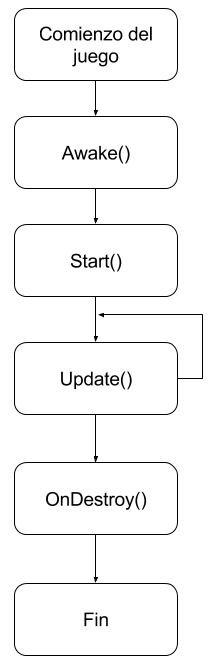
\includegraphics[width=0.5\textwidth]{unity-lifecycle.png}
    \caption{Versión simplificada del ciclo de vida de \emph{Unity}.}
	\label{fig:unity-lifecycle}
\end{figure}

El método \emph{Update} fue elegido para leer datos de los sensores. El problema que esto traía era que dicho método no puede ser bloqueado, ya que el ciclo principal de \emph{Unity} se ejecuta en un único \emph{thread} de procesamiento. \emph{Update} debe procesar información rápidamente para que el motor continue con su ciclo de actualizado y renderizado. Ante esta limitación, se decidió que los sensores operen en otros \emph{threads}. De esta forma, distintas rutinas podían leer y procesar información de los sensores y el juego luego podía obtener dicha información en los \emph{Update}. La arquitectura descrita se aplicó a la lectura y procesamiento de todas las señales elegidas, la cual se puede observar en la figura \ref{fig:architecture}.

\begin{figure}[H]
	\centering
    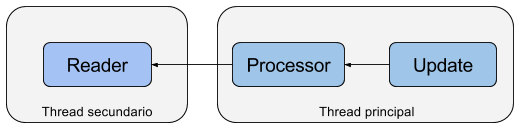
\includegraphics[width=0.5\textwidth]{architecture.png}
    \caption{Arquitectura utilizada en los universos 3D.}
	\label{fig:architecture}
\end{figure}

Para cada sensor, se cuenta con una instancia de la clase \emph{Reader} correspondiente, que es el encargado de obtener los datos del mismo. Esta instancia se ejecuta en otro \emph{thread}, ya que las operaciones de lectura son bloqueantes. Dicha instancia coloca los datos obtenidos por el sensor en una cola. Luego, una instancia de la clase \emph{Processor} puede consumir esos datos desde el \emph{thread} principal del juego. \emph{Processor} cuenta con un método \emph{Update}, el cual es llamado desde el ciclo del juego, es decir, desde el método \emph{Update} de la rutina que se ejecuta en \emph{Unity}. Cada vez que se llama a \emph{Update}, el procesador obtiene datos de la cola del lector (la deja vacía), los procesa y los deja disponibles para que el método \emph{Update} de \emph{Unity}, los pueda utilizar sin problemas. Es decir, en cada actualización se obtienen todos los datos no procesados en la actualización anterior y se procesan. Cabe destacar que \emph{Unity} no permitía el uso de la \emph{ConcurrentQueue} de \emph{.NET} (cola de datos que permite operaciones concurrentes), ya que utiliza una versión desactualizada de la plataforma. Por este motivo, se realizó una implementación propia. Ésta arquitectura nos permitió a su vez, desarrollar una aplicación en \emph{C\#}, por fuera de \emph{Unity}, con el fin de realizar pruebas y registrar sesiones de entrenamiento.

En todos los universos desarrollados se buscó que el uso de las bioseñales tenga sentido y no sea forzado. Es decir, que sea lógico y cómodo para el usuario. Se buscó que mejoren la experiencia, en lugar de empeorarla. Si la predicción fallara y el usuario se encontrara realmente en otro estado, se buscó que esta situación no perjudique al usuario. Es decir, que no le quite vida o decremente sus posibilidades de ganar. En el peor caso, que beneficie al usuario, en lugar de perjudicarlo.

\subsection{Universo 3D Utilizando Bioseñales Cerebrales}

Se desarrolló un vídeojuego de terror en el que el usuario debía escaparse de un laberinto. Dicho laberinto es oscuro, está custodiado por \emph{Zombies} (criaturas hostiles que atacan al jugador al verlo) y hay bombas escondidas. El usuario cuenta con una pistola y los movimientos se controlan utilizando el teclado y el \emph{mouse}. Como se mencionó anteriormente, se utilizaron ondas cerebrales para detectar si el usuario se encontraba con los ojos abiertos o cerrados. En este videojuego, cuando el usuario cierra los ojos y no realiza movimientos, puede escuchar los sonidos que generan las bombas y las puede visualizar en la pantalla luego de abrir los ojos, para poder desactivarlas. A su vez, se acumula el tiempo que el usuario se encuentra con los ojos cerrados, y luego de abrir los ojos, se puede observar a los \emph{Zombies}, bombas, municiones y paquetes de salud  a través de las paredes. Este habilidad dura tantos segundos como los acumulados con los ojos cerrados, hasta un valor máximo de 10 segundos. El personaje puede escuchar y visualizar bombas, \emph{Zombies}, entre otros, ya que al cerrar los ojos, se concentra e incrementa la sensibilidad auditiva. Aumentar los sentidos es un recurso muy utilizado en muchos videojuegos. La diferencia es que en este videojuego, el usuario realmente se encuentra con los ojos cerrados por lo que se utiliza el estado actual en lugar de un simple botón. Sin embargo, al estar con los ojos cerrados, corre el riesgo de ser atacado y no poder responder a tiempo. En la figura \ref{fig:eeg-screen-shot} se puede observar una captura de pantalla que muestra lo que ve el usuario al abrir los ojos luego de haberlos mantenido cerrados por unos segundos.

\begin{figure}[H]
	\centering
    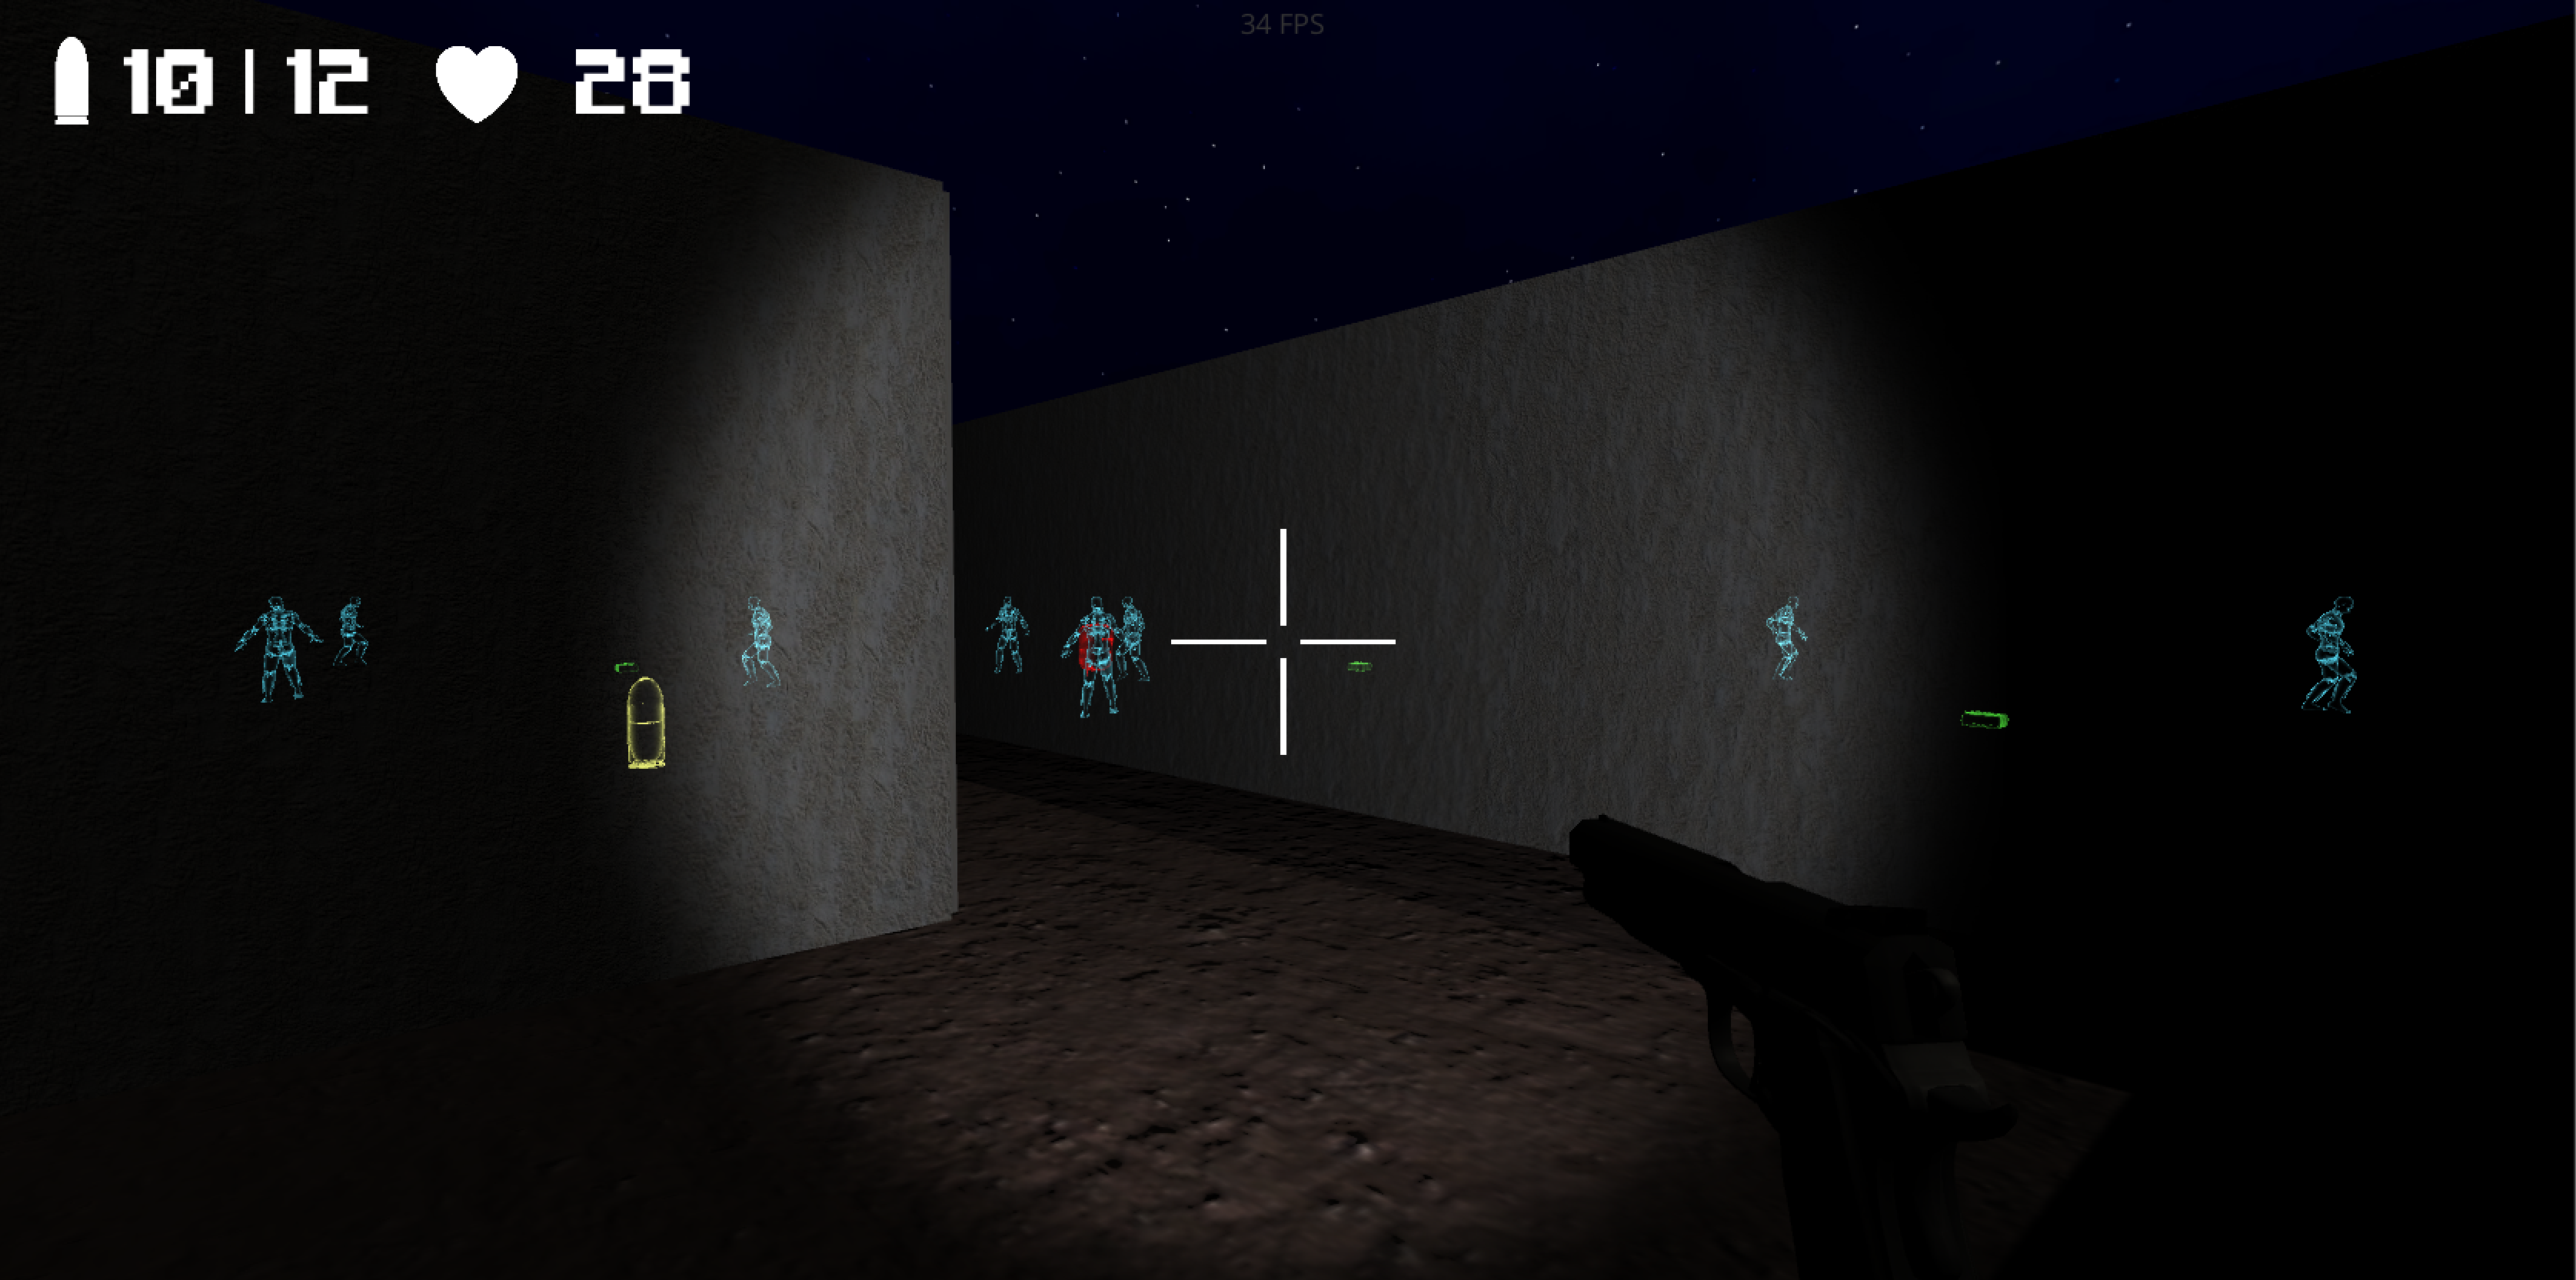
\includegraphics[width=0.8\textwidth]{eeg-screen-shot.png}
    \caption{Captura de pantalla del universo desarrollado para el dispositivo \acrshort{eeg}. Aquí se observa el resultado de mantener los ojos cerrados durante algunos segundos.  Los elementos verdes son bombas, los cyan \emph{Zombies}, los amarillos municiones y los rojos paquetes de salud.}
	\label{fig:eeg-screen-shot}
\end{figure}

La clase \emph{EEGProcessor} se encarga de obtener lecturas del cerebro de una cola. Dicha cola se encuentra en \emph{EEGReader} y es esta clase la que se encarga de leer los datos del sensor y publicarlos a la cola. \emph{EEGProcessor} permite que se especifique una lista de funciones a las cuales llamar una vez que se procesaron los datos. Luego de obtener $256$ lecturas de cada electrodo, se calcula la \acrshort{fft} para cada electrodo. Es en este instante en el que se llama a dichas funciones. De esta manera, una rutina en \emph{Unity} es llamada y obtiene la información necesaria del procesador en ese instante. En este caso, el estado de los ojos. En otras palabras, cuando el procesador tiene información para enviar, le notifica a la rutina de \emph{Unity} para que éste la utilice.

Como se utilizó reconocimiento de patrones, se implementó una interfaz para entrenar al clasificador. Dicho entrenamiento tiene una duración de entre $1$ y $10$ minutos (determinable por el usuario) , en los cuales se le indica al usuario que abra y cierre los ojos por períodos de tiempo aleatorio. Durante el entrenamiento se identifica el estado en el que está el usuario. Una vez finalizado el entrenamiento, el usuario puede comenzar a jugar.

Debido a que la precisión del clasificador era de un  $75\%$ (como se verá en la sección \ref{sec:eeg-results}), se decidió establecer un umbral para determinar en que momento el usuario se encuentra con los ojos cerrados. Cada vez que se predice que se encuentra con los ojos abiertos, se decrementa un contador, y cada vez que se predice que se encuentra con los ojos cerrados, se incrementa. El contador tiene como valor mínimo cero y el valor máximo es establecido por el usuario.  Luego, cuando el contador supera un umbral, se considera que los ojos están cerrados hasta que dicho contador se encuentre nuevamente por debajo del umbral o hasta que el usuario realice movimientos con el personaje. Al procesar las ondas cerebrales, se observó, que en ocasiones, aún cuando el usuario se encontraba con los ojos abiertos, las ondas \emph{Alfa}, obtenían valores muy altos. Por este motivo, podían ser clasificadas como ojos cerrados. Al utilizar un umbral, se impone la condición de que las ondas  \emph{Alfa} se encuentren elevadas por un determinado periodo de tiempo. Algo que no debería suceder al encontrarse con los ojos abiertos. Este comportamiento se controla con dos variables (umbral mínimo y umbral máximo) accesibles desde el menú de pausa. Si se identifica que el usuario registra valores de \emph{Alfa} elevados por períodos de una duración de tiempo determinada, se deben incrementar  tanto el umbral mínimo, como el máximo. En caso contrario, se deben decrementar. La utilización de este sistema, puede causar retardo en la detección de estado ya que se debe esperar a tener una mínima cantidad de lecturas de datos para determinar el estado. Por este motivo, se debió tomar una decisión de compromiso en el momento de elegir los valores. No debían ser muy bajos, ya que se iba a detectar falsamente que el usuario se encontraba con los ojos cerrados. Pero tampoco, debían ser muy altos porque el retardo iba a ser elevado. Como el usuario debe esperar al menos tantos segundos como especifique el umbral (pues las ventanas de muestras son de $1$ segundo), se decidió sumar el valor del umbral mínimo a la cantidad de segundos acumulados.

\subsection{Universo 3D Utilizando Bioseñales de los Músculos}

Se desarrolló un universo 3D interactivo en el que el usuario al tensar el músculo acumula energía. Luego, al liberar la tensión, envía un proyectil eléctrico que impacta contra otros objetos. Cuanto mayor sea el tiempo que se mantiene tensión, mayor es la fuerza del proyectil y mayor es la energía liberada en el impacto contra otros objetos. En el universo 3D se cuenta, por ejemplo, con barriles colocados uno encima del otro. Dichos barriles pueden ser derrumbados arrojando proyectiles. Se decidió utilizar la tensión para este tipo de ataque ya dentro de la simulación, los proyectiles se crean desde el el brazo y mano del jugador virtual. En la figura \ref{fig:emg-screenshot} se puede observar una captura de pantalla de dicho universo.

\begin{figure}[H]
	\centering
    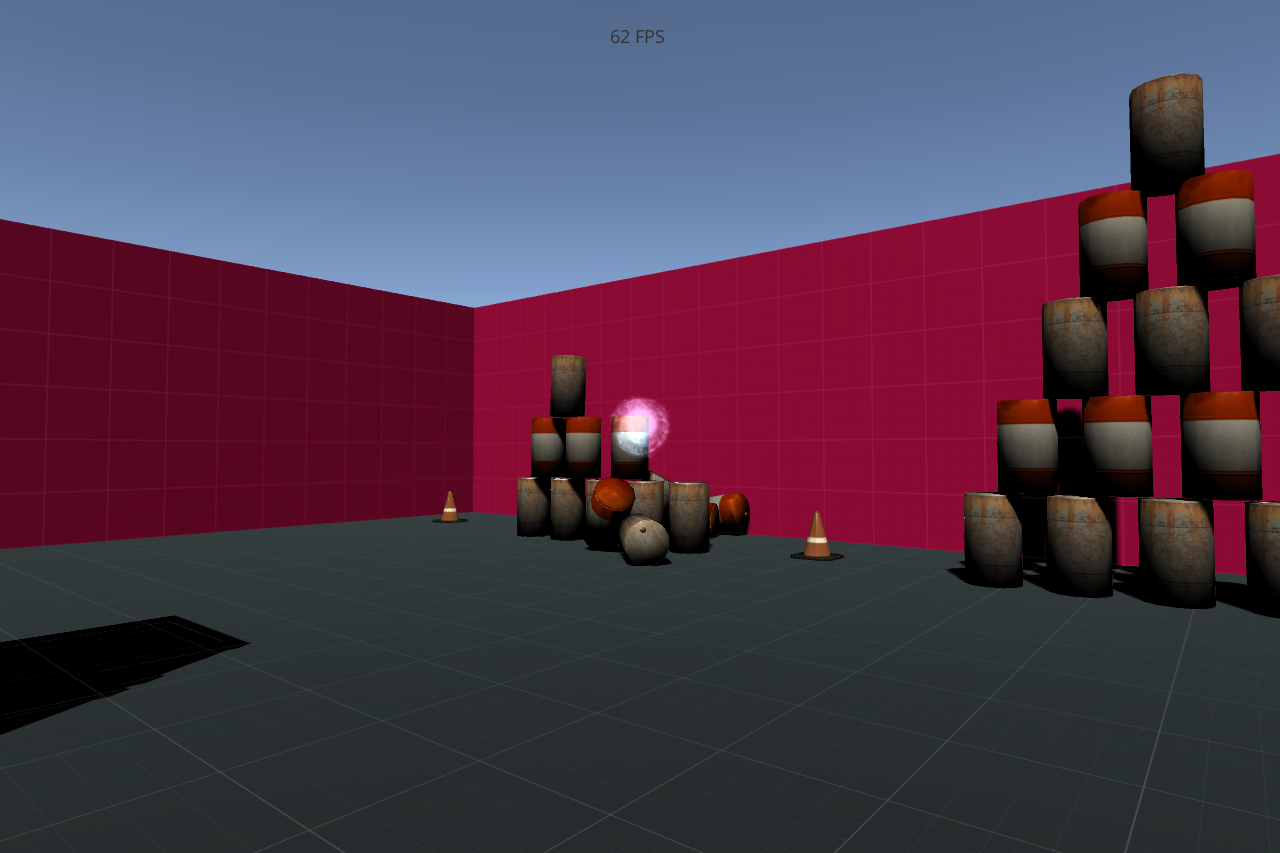
\includegraphics[width=0.8\textwidth]{emg-screenshot.png}
    \caption{Captura de pantalla del universo desarrollado para el dispositivo \acrshort{emg}.}
	\label{fig:emg-screenshot}
\end{figure}


La fuerza se modeló como un simple contador. Cada actualización en la que el músculo se encuentra tenso, se incrementa el contador. Si se encuentra relajado, se decrementa el contador. Dicho contador nunca alcanza valores menores a $0$ y nunca valores mayores a un máximo establecido anteriormente. Una vez que el contador supera un umbral, si se detecta una relajación, se libera el proyectil cargado. Se puede observar una pequeña latencia al liberal el proyectil. Esto se debe a que, como se utilizan $128$ muestras para extraer las características y predecir un estado, se obtienen cambios de estado cada cuarto de segundo. La velocidad y tamaño del proyectil lanzado son proporcionales a el valor del contador, por lo que hay un incentivo para mantener el músculo tensado por una mayor cantidad de tiempo.

Al igual que con la simulación que utiliza información del \acrshort{eeg}, aquí se cuenta con un lector y un procesador. El procesador también permite que otros objetos se subscriban a eventos. Cuando el procesador obtuvo la cantidad de muestras necesarias y las procesó, notifica a los objetos que se hayan suscrito. De esta manera, la rutina que se ejecuta en \emph{Unity} puede conocer el estado en cada actualización y realizar las acciones necesarias. Aquí no hizo falta la utilización de un umbral para determinar un cambio de estado, ya que la precisión era muy alta. Este universo también cuenta con una interfaz con instrucciones de entrenamiento.

\subsection{Universo 3D Utilizando el Ritmo Cardíaco}

Se continuó con el desarrollo del videojuego en el que se utilizaron las bioseñales del cerebro. Se desarrolló un nuevo nivel que sucede luego de que el jugador escape del laberinto. Al escapar del laberinto, éste se encuentra en el centro de un campo,  con una linterna y un arma, rodeado de \emph{Zombies}. El objetivo es sobrevivir a todas las olas de ataques de \emph{Zombies}. Cuando el jugador comienza a ponerse nervioso, el ritmo cardíaco aumenta. Se utiliza esta información para simular el temblor de las manos del jugador virtual. Cuanto más alto es el ritmo cardíaco, más movimientos aleatorios realiza el arma, dificultando la tarea de apuntar. Este movimiento imita a la realidad, ya que cuando uno se encuentra nervioso, le resulta más difícil realizar acciones con las manos, como apuntar un arma. El jugador puede también quedarse sin municione, lo que genera mayor nerviosismo en el usuario porque no cuenta con ninguna forma de defenderse. En la figura \ref{fig:spo2-screenshot} se puede observar una captura de pantalla del universo desarrollado.

\begin{figure}[H]
	\centering
    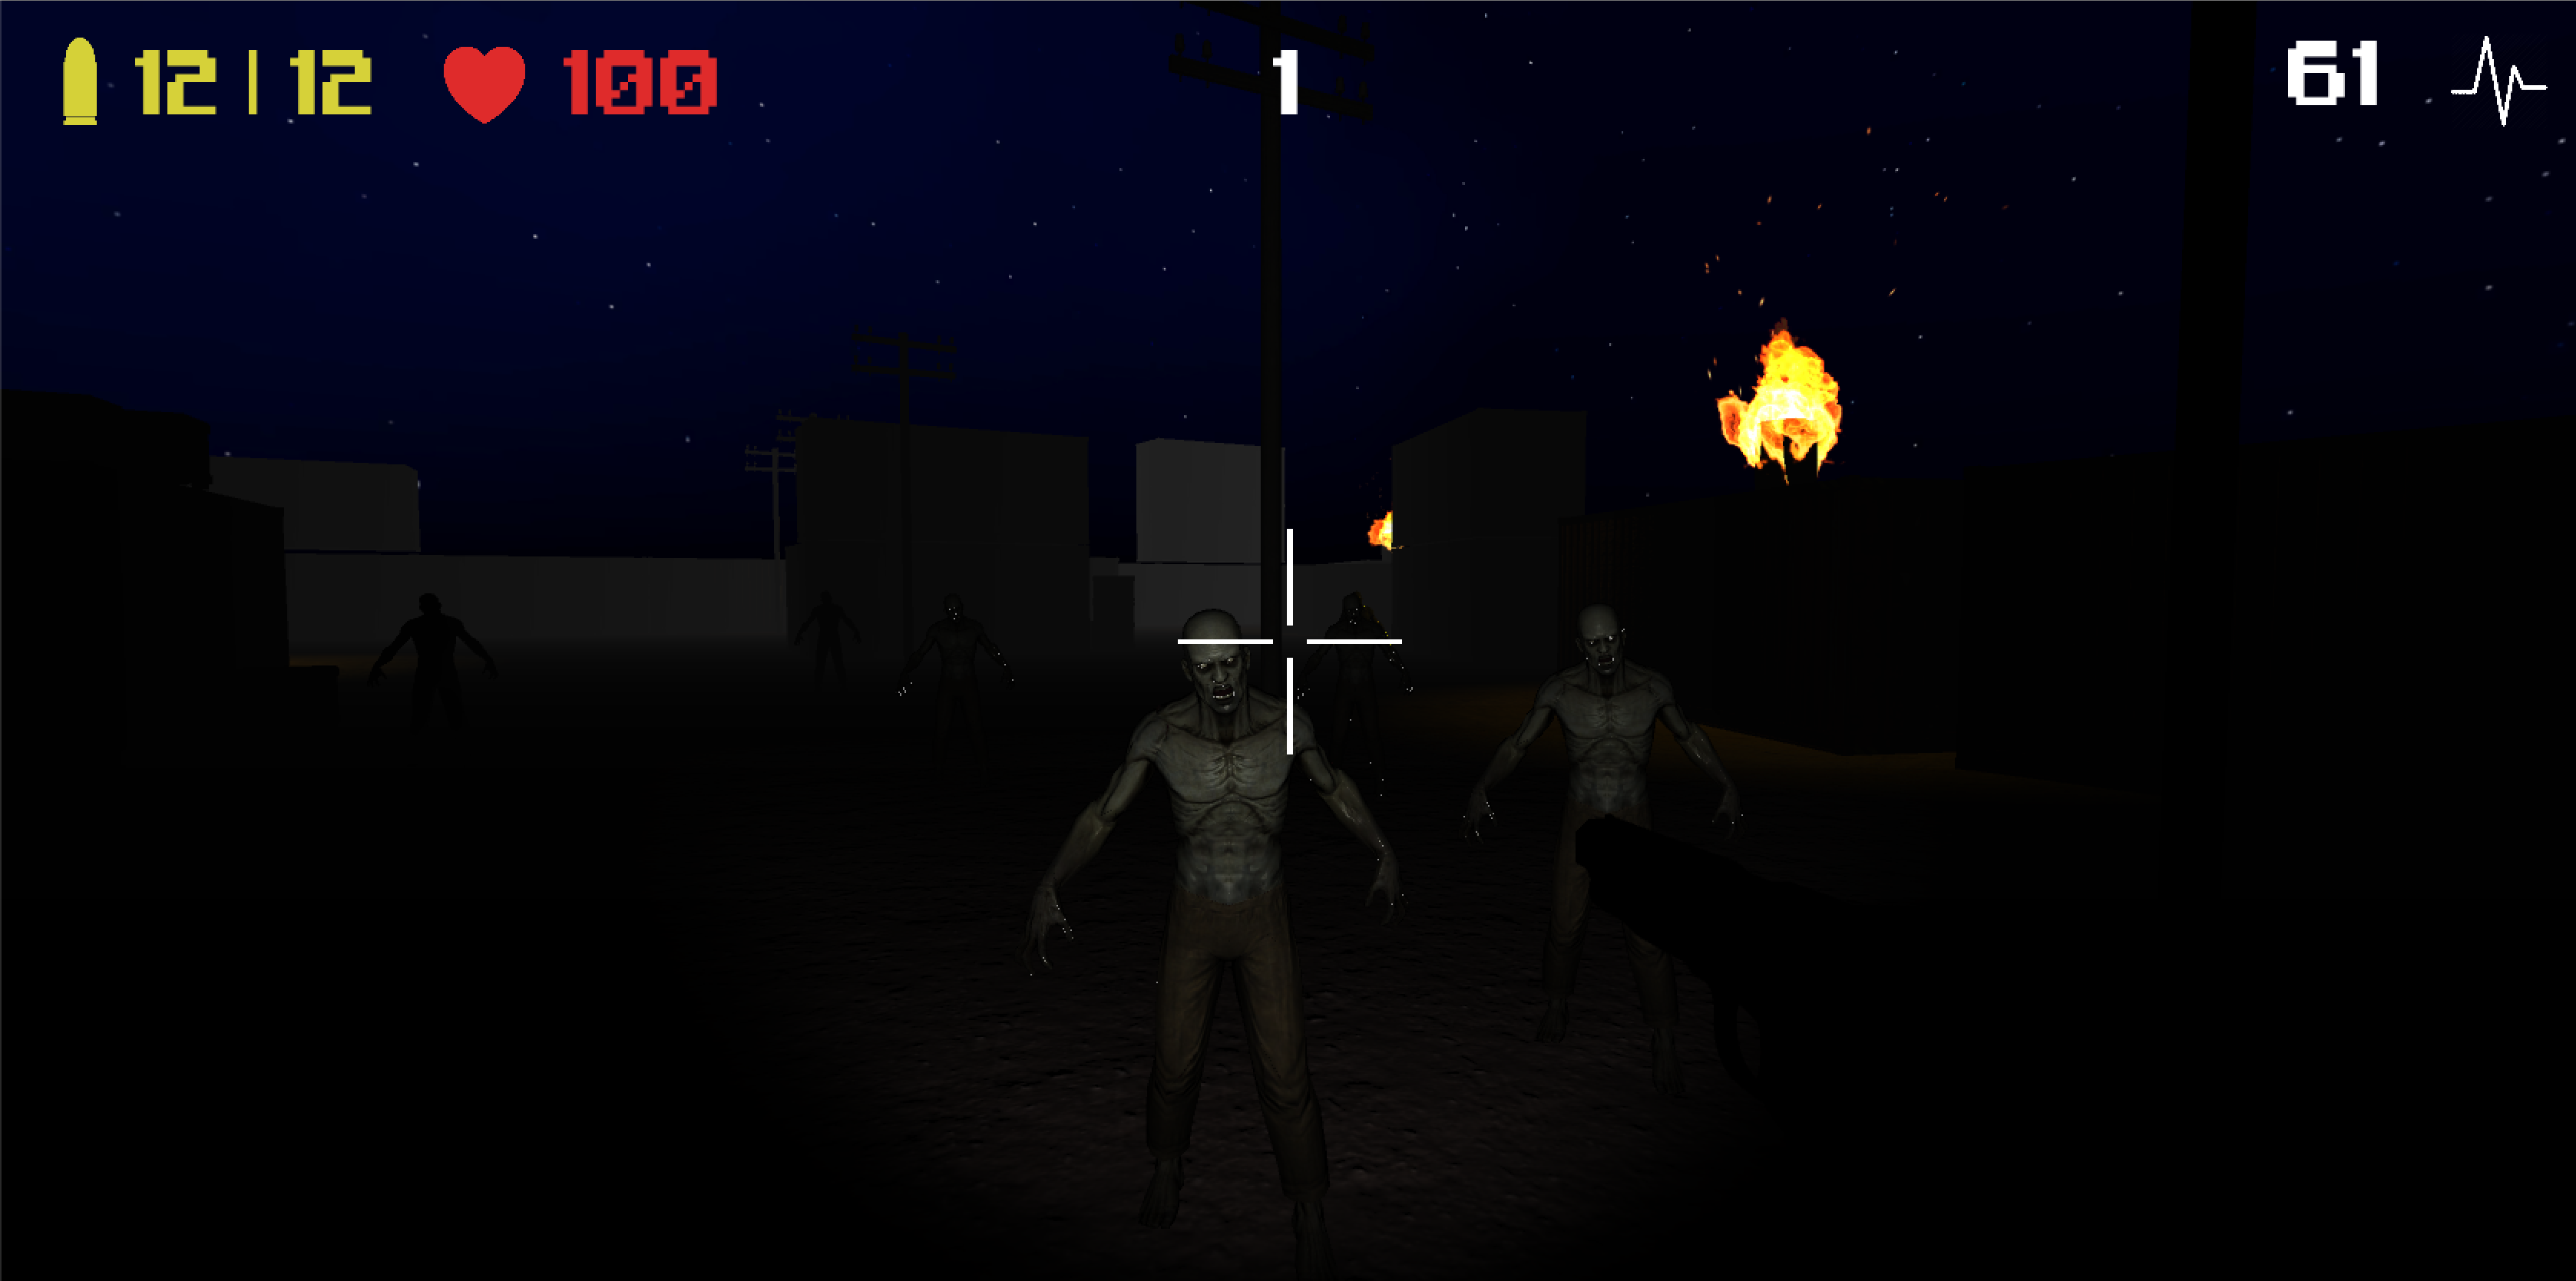
\includegraphics[width=0.8\textwidth]{spo2-screenshot.png}
    \caption{Captura de pantalla del universo desarrollado para el dispositivo \acrshort{spo2}. En la esquina superior derecha se puede observar el ritmo cardíaco del usuario.}
	\label{fig:spo2-screenshot}
\end{figure}

Aquí también se cuenta con un procesador (\emph{SPO2Processor}) y un lector (\emph{SPO2Reader}). El procesador expone un método que permite obtener el ritmo cardíaco actual. De esta manera, la rutina en \emph{Unity} obtiene este valor en cada actualización y en base a él, realiza movimientos sobre la cámara. Dichos movimientos se modelaron utilizando funciones trigonométricas para que sean armónicas y agradables a la vista. La magnitud de los movimientos se controla con dos variables: mínimo y máximo. Una establece el umbral mínimo que se utiliza para determinar si el usuario está nervioso y la otra el máximo. Luego, si el el ritmo cardíaco es mayor al umbral mínimo, se interpola linealmente entre el mínimo y el máximo.

\section{Arquitectura de la librería implementada}

El proyecto desarrollado sigue la estructura clásica de un proyecto \emph{Unity}. Se cuenta con el directorio \emph{Assets}, que contiene imágenes, archivos de audio, y archivos de código que forman parte del proyecto. Dentro de este directorio, se decidió separar los archivos relacionados a las simulaciones interactivas, y los archivos relacionados a la lectura y procesamiento de las bioseñales. El directorio \emph{pf-core} contiene todas las clases y rutinas necesarias para poder establecer una conexión con los sensores, procesar los datos leídos, y exponer los resultados para que puedan ser utilizados en otras aplicaciones.

Como se mencionó en la sección \ref{sec:unity-net}, la plataforma \emph{.NET} utiliza código \acrshort{cil} como representación intermedia, que puede ser ejecutado en una maquina virtual. El código \emph{CIL} puede ser almacenado como un archivo ejecutable (por ejemplo, un archivo \emph{.exe} para \emph{Windows}), o como una librería dinámica (por ejemplo, \emph{.dll}). En el caso de nuestro proyecto, sería fácil generar un archivo \emph{.dll} a partir del directorio \emph{pf-core}, que luego podría ser utilizado en otros proyectos. Por ejemplo, si se quisiera crear una aplicación que registre el ritmo cardíaco de un paciente durante un intervalo de tiempo y luego almacene los resultados en un archivo, se podría incluir nuestra librería \emph{.dll} para poder acceder al sensor \acrshort{spo2}.

\addcontentsline{toc}{chapter}{Bibliografía}
\bibliography{bibliography}{}
\bibliographystyle{babplain}
 
\end{document}